
\documentclass[a4paper,12pt]{article}
\usepackage{graphicx}
\usepackage[table,xcdraw]{xcolor}
\usepackage{geometry}
\usepackage{float}
\usepackage[colorlinks=false, hidelinks]{hyperref}
\usepackage{fancyhdr}% For page numbering
\geometry{top=1in,bottom=1in,left=1in,right=1in}
\usepackage{listings}
\usepackage{xcolor}
\usepackage{hyperref}
\pagestyle{empty}


\begin{document}

\begin{center}
    \vspace{0.2cm}
    \textbf{\large{Course Title: Software Engineering \& ISD Lab}}\\
    \vspace{0.2cm}
    \textbf{Course Code: CSE-404}\\
    \vspace{0.2cm}
    \textbf{4\textsuperscript{th}Year 1\textsuperscript{st}Semester Examination 2023}\\
    \vspace{0.5cm}
    \textbf{Date of Submission: \today}\\

    \vspace{1.5cm}
    
\includegraphics[width=0.35\textwidth]{images/logo.png}\\ % Replace 'logo.png' with the correct path if you have the university logo image
    \vspace{1cm}

    \textbf{Submitted to}\\
    \vspace{0.2cm}
    \textbf{\href{https://juniv.edu/teachers/musfique.anwar}{Dr. Md Musfique Anwar}}\\
    {Professor}\\
    \vspace{0.2cm}
    \textbf{\href{https://juniv.edu/teachers/hkabir}{Dr. Md. Humayun Kabir}}\\
    {Professor}\\


    \vspace{1cm}

    \begin{table}[h!]
        \centering
        \arrayrulecolor{black}
        \begin{tabular}{|c|c|c|c|}
            \hline
            \rowcolor[HTML]{2F4F4F} % Changed header background color to dark slate gray
            {\color[HTML]{FFFFFF}\textbf{Sl}}& {\color[HTML]{FFFFFF}\textbf{Class Roll}}& {\color[HTML]{FFFFFF}\textbf{Exam Roll}}& {\color[HTML]{FFFFFF}\textbf{Name}}\\ \hline
            \rowcolor[HTML]{B0E0E6}
            \textbf{1}& \textbf{408} & \textbf{202220} & \textbf{Sudipta Singha} \\ \hline

        \end{tabular}
    \end{table}

    \vspace{1cm}

    Department of Computer Science and Engineering\\
    Jahangirnagar University\\
    Savar, Dhaka, Bangladesh\\
\end{center}

\newpage

\tableofcontents

\newpage
\pagestyle{fancy}
\fancyhf{}
\fancyfoot[C]{\thepage} % Page number in the center of the footer
\section{Introduction}

The Jahangirnagar University Medical Center Management System project was designed to streamline and
digitalize the management of the university’s medical center. This system aimed to provide essential features
such as user registration, appointment scheduling, inventory tracking for the medical store, and the
publication of informational vlogs on seasonal diseases. The project’s primary objective was to enhance
efficiency, improve accessibility for users, and ensure better management of medical resources. 
During my involvement, the project achieved several milestones, including a functional user authentication
system, a dynamic dashboard for doctors, lab technician, storekeeper users, and the successful integration of ambulance driver details for emergency services. The project utilized Django as the backend framework, ensuring a robust and scalable system.
. Github link for the project is provided here
\begin{figure}[H]
    \centering
    
\includegraphics[width=0.5\textwidth]{images/simple_prcode.png}
    \caption{QR code for the project link}
    \label{fig:qrcode}
\end{figure}
\textbf{Features}
\begin{itemize}
    \item Sign Up
    \item Log In
    \item See the information of waiting patients
    \item Prescribe medicines and test for a patient
    \item Dispense medicines to patients
    \item Update stock information
    \item Certify patients for fund collection
    \item Publish information and preventative measures for seasonal diseases
    \item Schedule appointment for doctors and lab tests
    \item Collect test reports and Prescriptions
    \item Reschedule test appointments
    \item Submit test reports
    \item Visit the seasonal diseases portal
\end{itemize}
\newpage
\section{My Contribution}
As an active team member, I contributed significantly to the development and implementation of various
features. Here are some statictics from github where we have been storing repository for JUMCMS.
\begin{figure}[H]
    \centering
    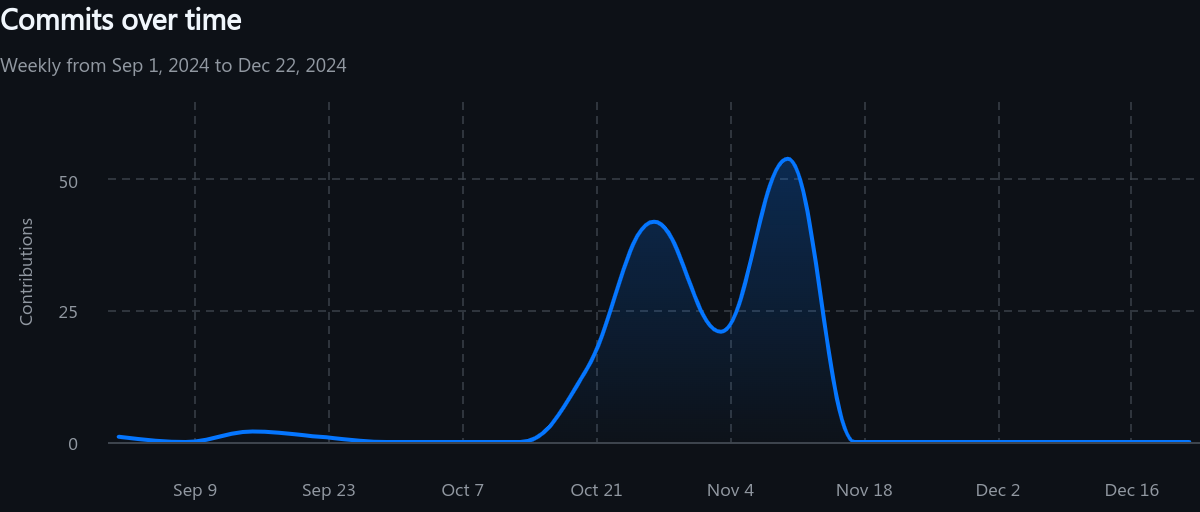
\includegraphics[width=0.8\textwidth]{images/Commits over time.png}
    \caption{Overall Commits}
    \label{fig:overallcommits}
\end{figure}
This figure shows the overall commits which are made by all members of the team. We have achieved 134 commits.
\begin{figure}[H]
    \centering
    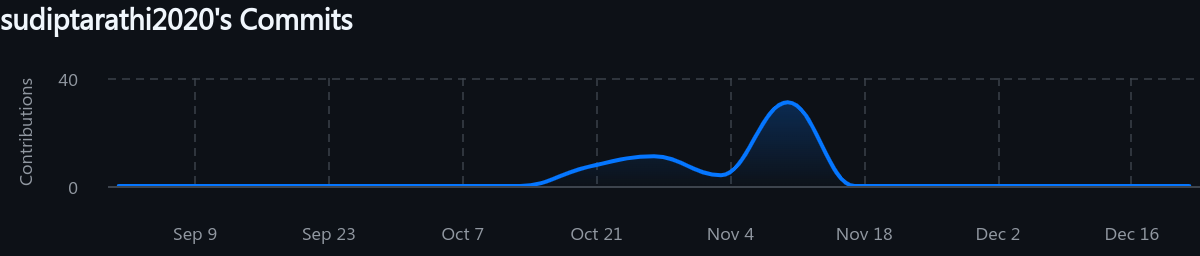
\includegraphics[width=0.8\textwidth]{images/sudiptarathi2020's Commits.png}
    \caption{Commits by me}
    \label{fig:mycommits}
\end{figure}
This figure shows the commits by me(sudiptarathi2020). I have made total of 53 commits in git. 
\begin{figure}[H]
    \centering
    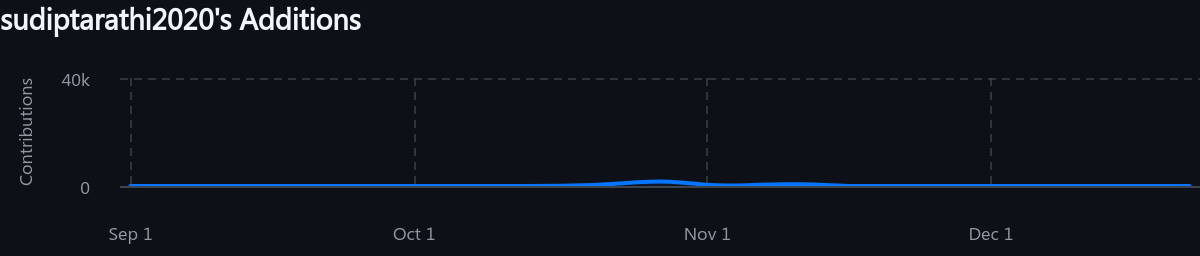
\includegraphics[width=0.8\textwidth]{images/sudiptarathi2020's Additions.png}
    \caption{Additions by me}
    \label{fig:myadditions}
\end{figure}
This figure shows the additions of line I have contributed to the project. I have made a total 2866 additions
into the projects codebase.
\newpage
\subsection{User Story}
I have been actively involved in writting the user story for JUMCMS.
\begin{itemize}
    \item Wrote user story for Dispense medicines to patients 
    \item Wrote user story for Account creation
    \item Wrote user story update stock information
    \item Participated in discussion with team members for other user stories
\end{itemize}
\begin{figure}[H]
    \centering
    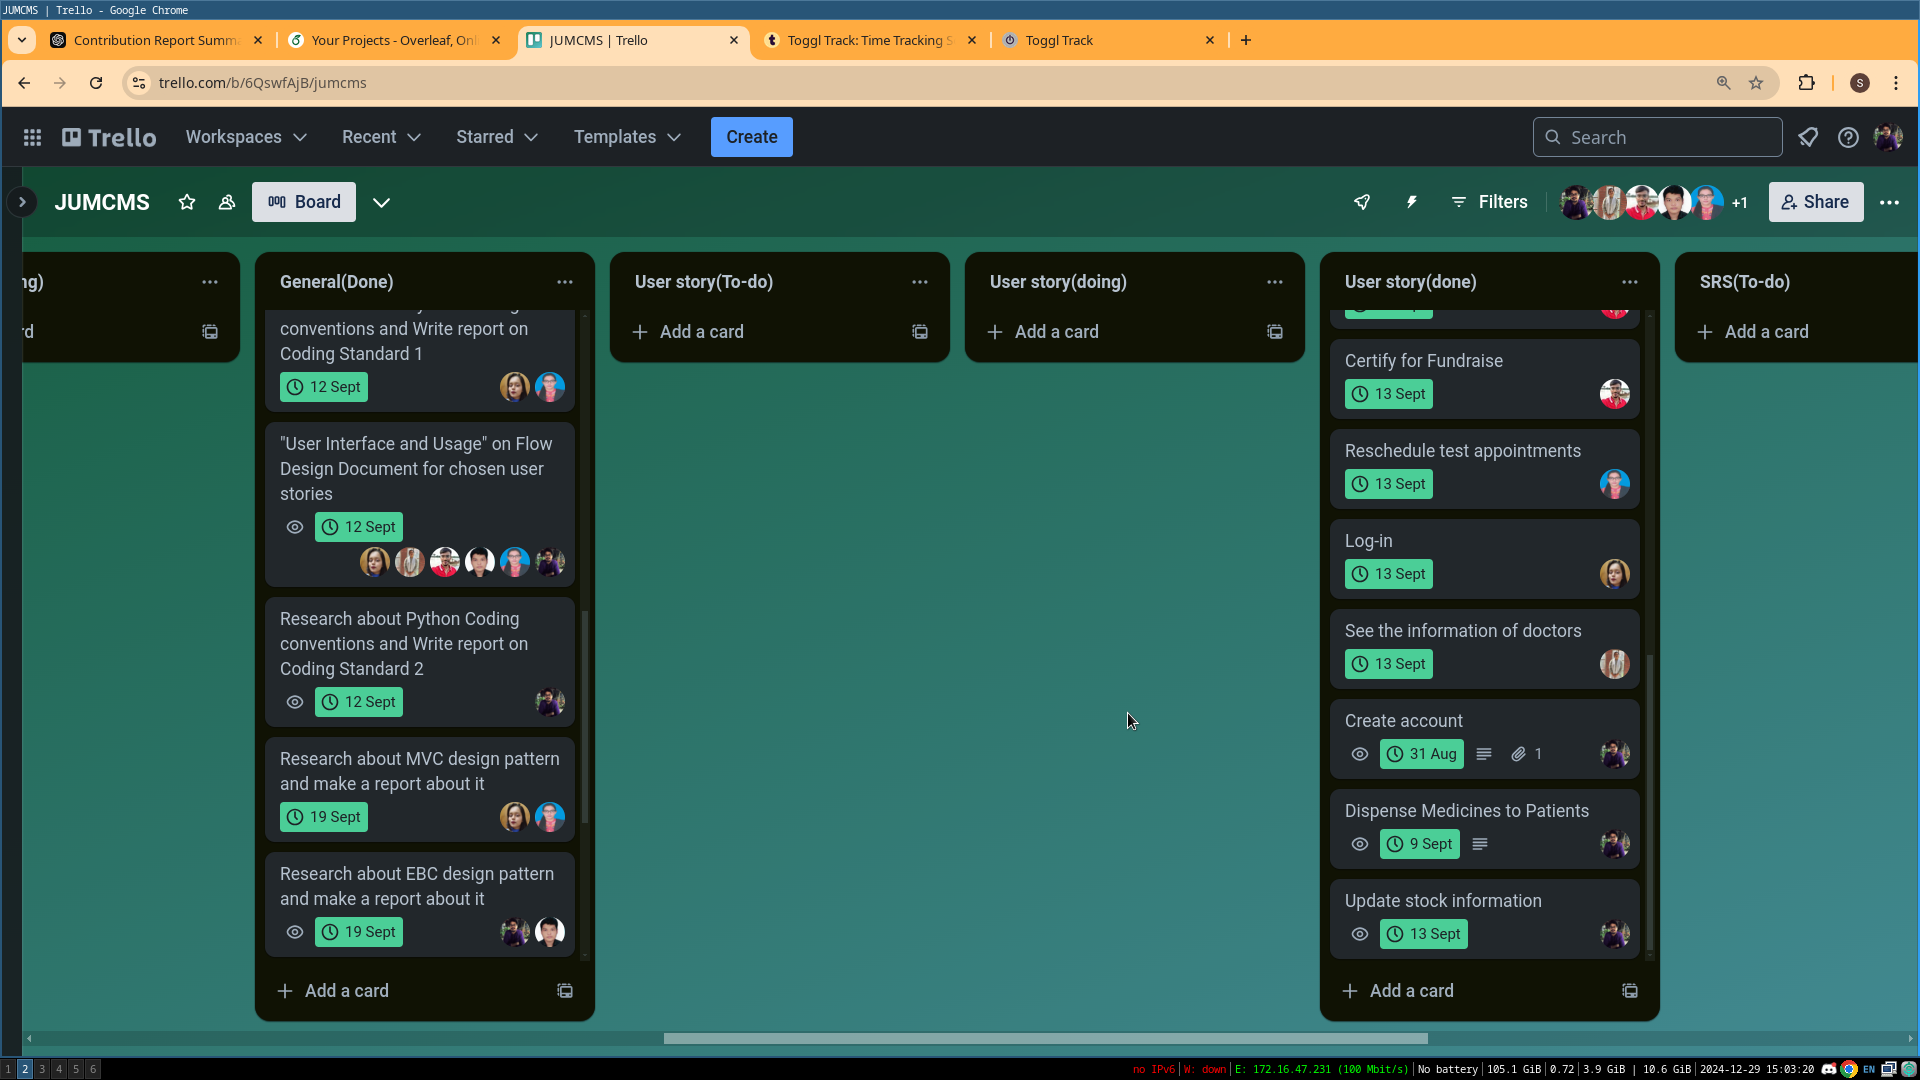
\includegraphics[width=0.8\textwidth]{images/trello_user_story.png}
    \caption{Trello work assignment}
    \label{fig:trellouserstory}
\end{figure}
\begin{figure}[H]
    \centering
    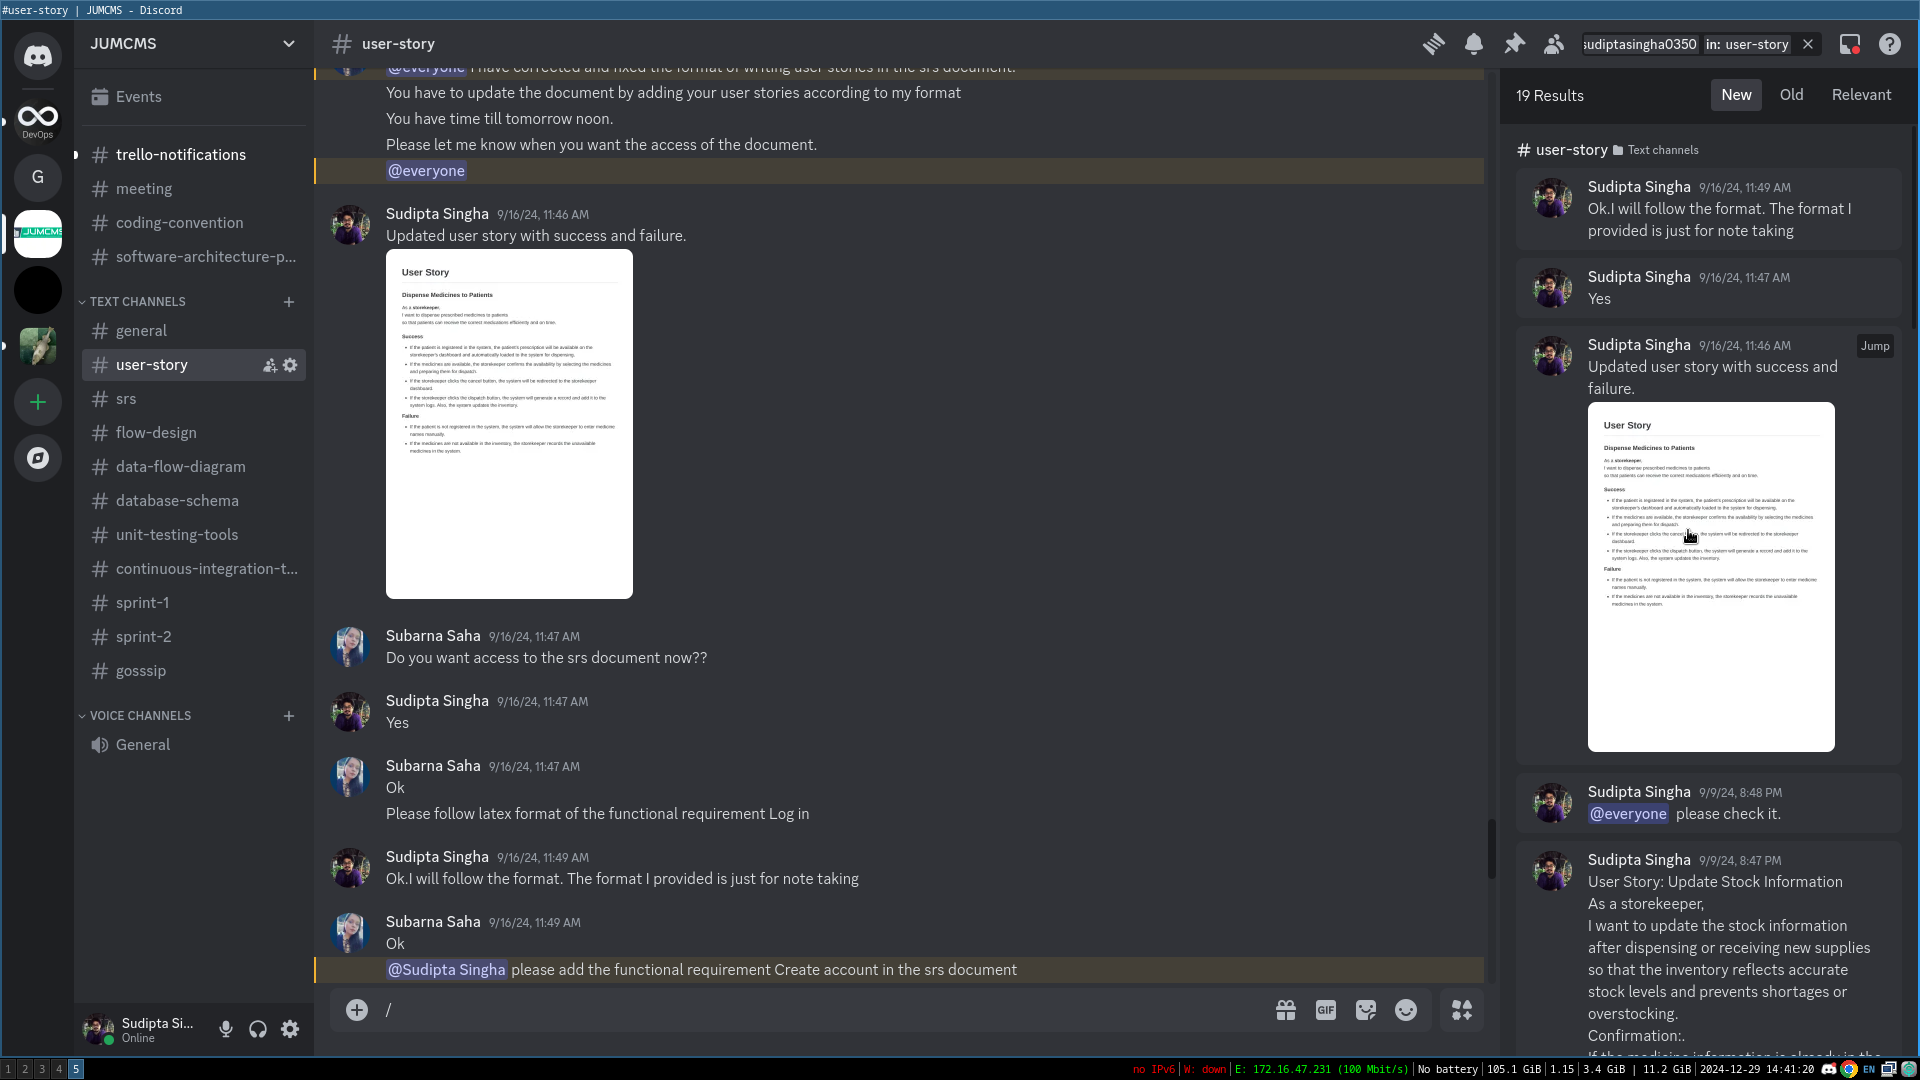
\includegraphics[width=0.8\textwidth]{images/discord_user_story.png}
    \caption{Discord Conversation in user story channel}
    \label{fig:discorduserstory}
\end{figure}

\subsection{SRS}
I have been assigned the task of writting users needs and risk definition in srs.
\begin{itemize}
    \item Wrote User needs in SRS
    \item Wrote Risk definition in SRS
    \item Wrote and help other team members in writting non-functional requirements
\end{itemize}
\begin{figure}[H]
    \centering
    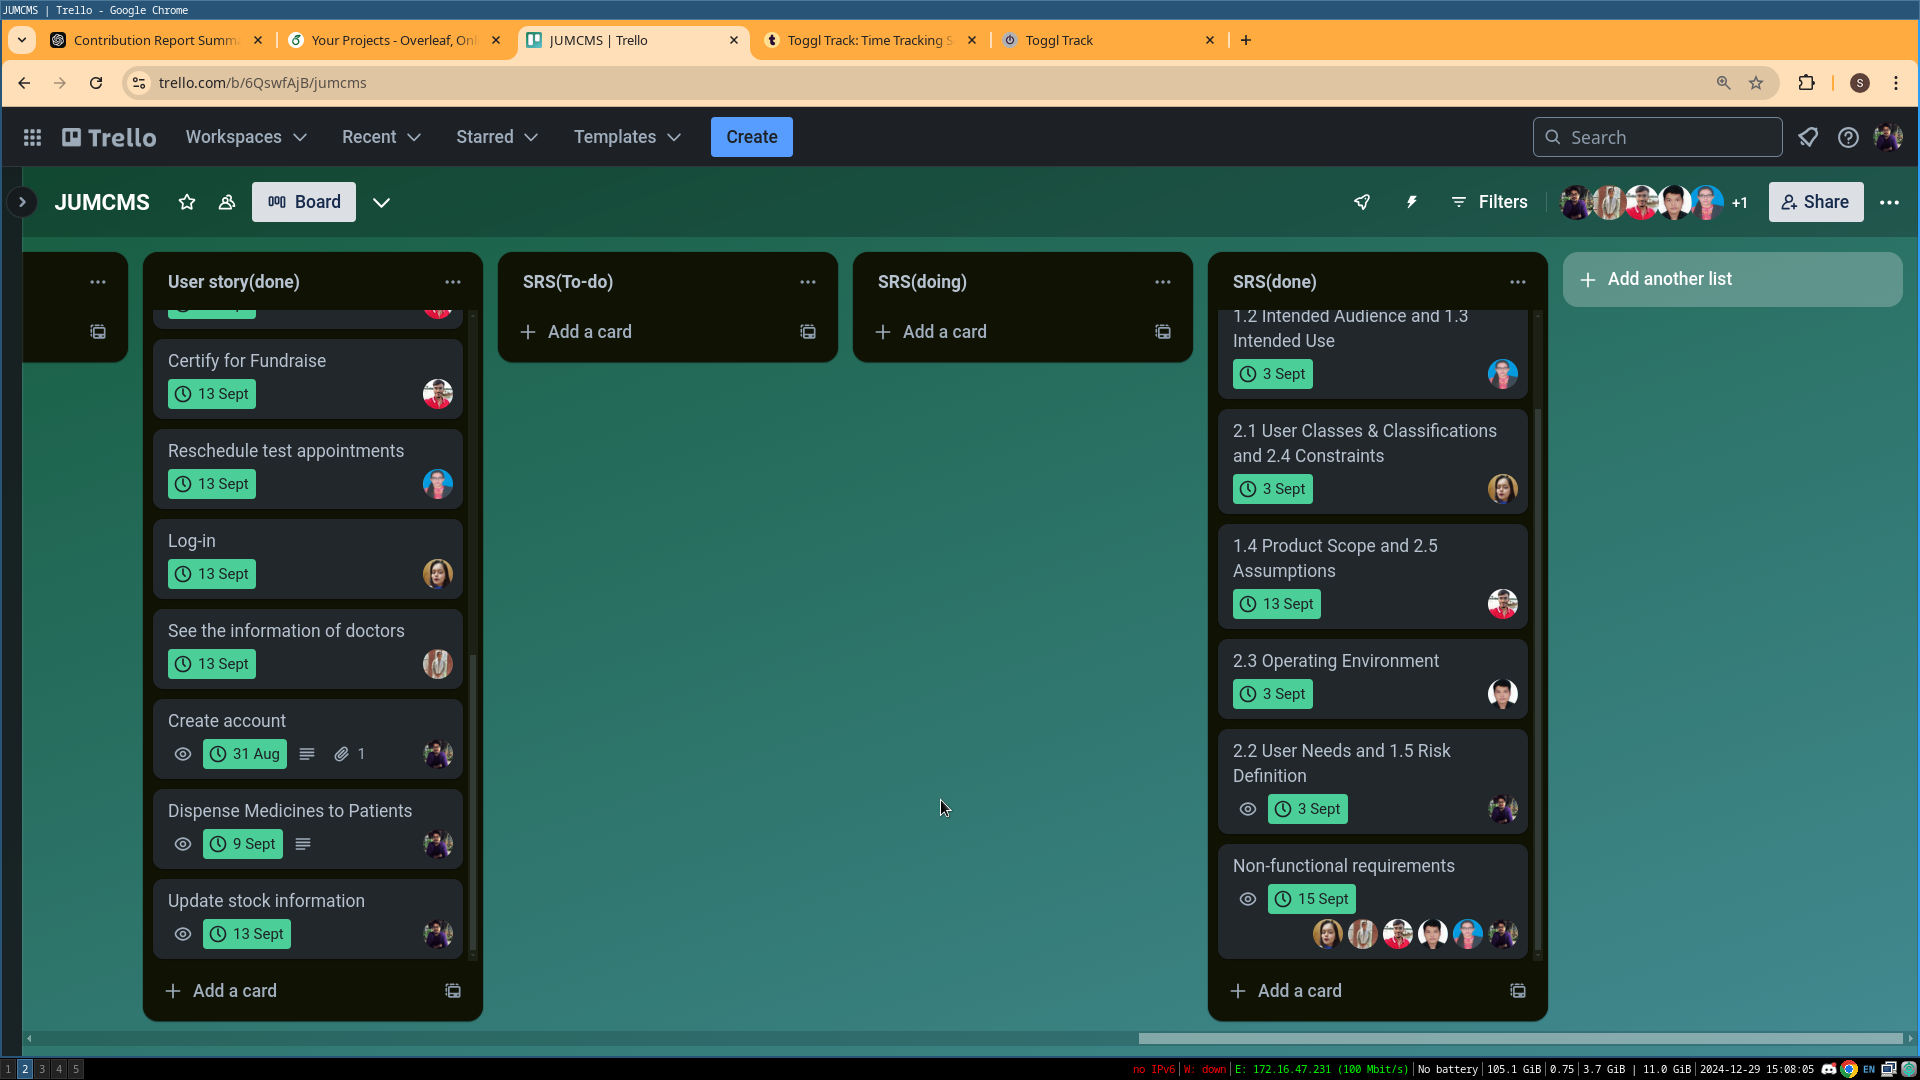
\includegraphics[width=0.8\textwidth]{images/trell_srs.png}
    \caption{Trello SRS assignment}
    \label{fig:trellosrs}
\end{figure}
\begin{figure}[H]
    \centering
    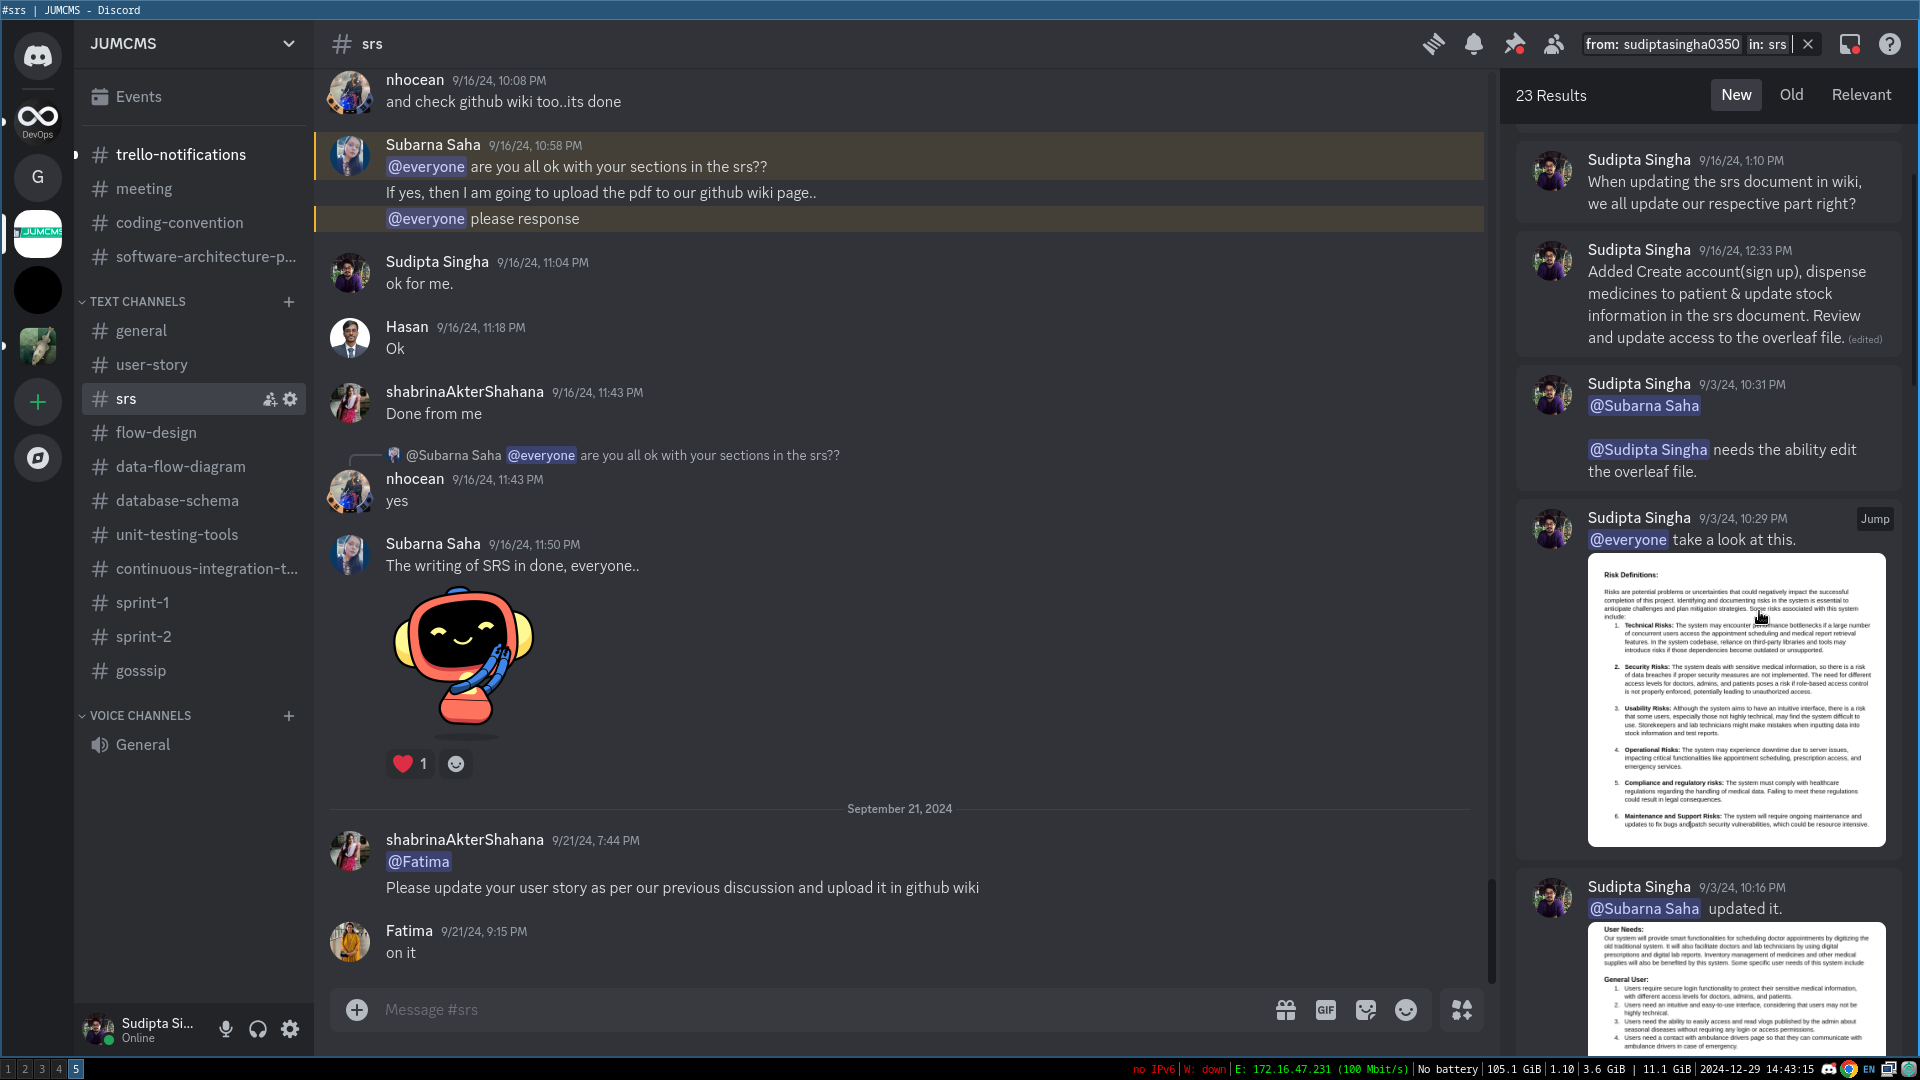
\includegraphics[width=0.8\textwidth]{images/discord_srs.png}
    \caption{Discord Conversation in SRS channel}
    \label{fig:discordsrs}
\end{figure}
\begin{figure}[H]
    \centering
    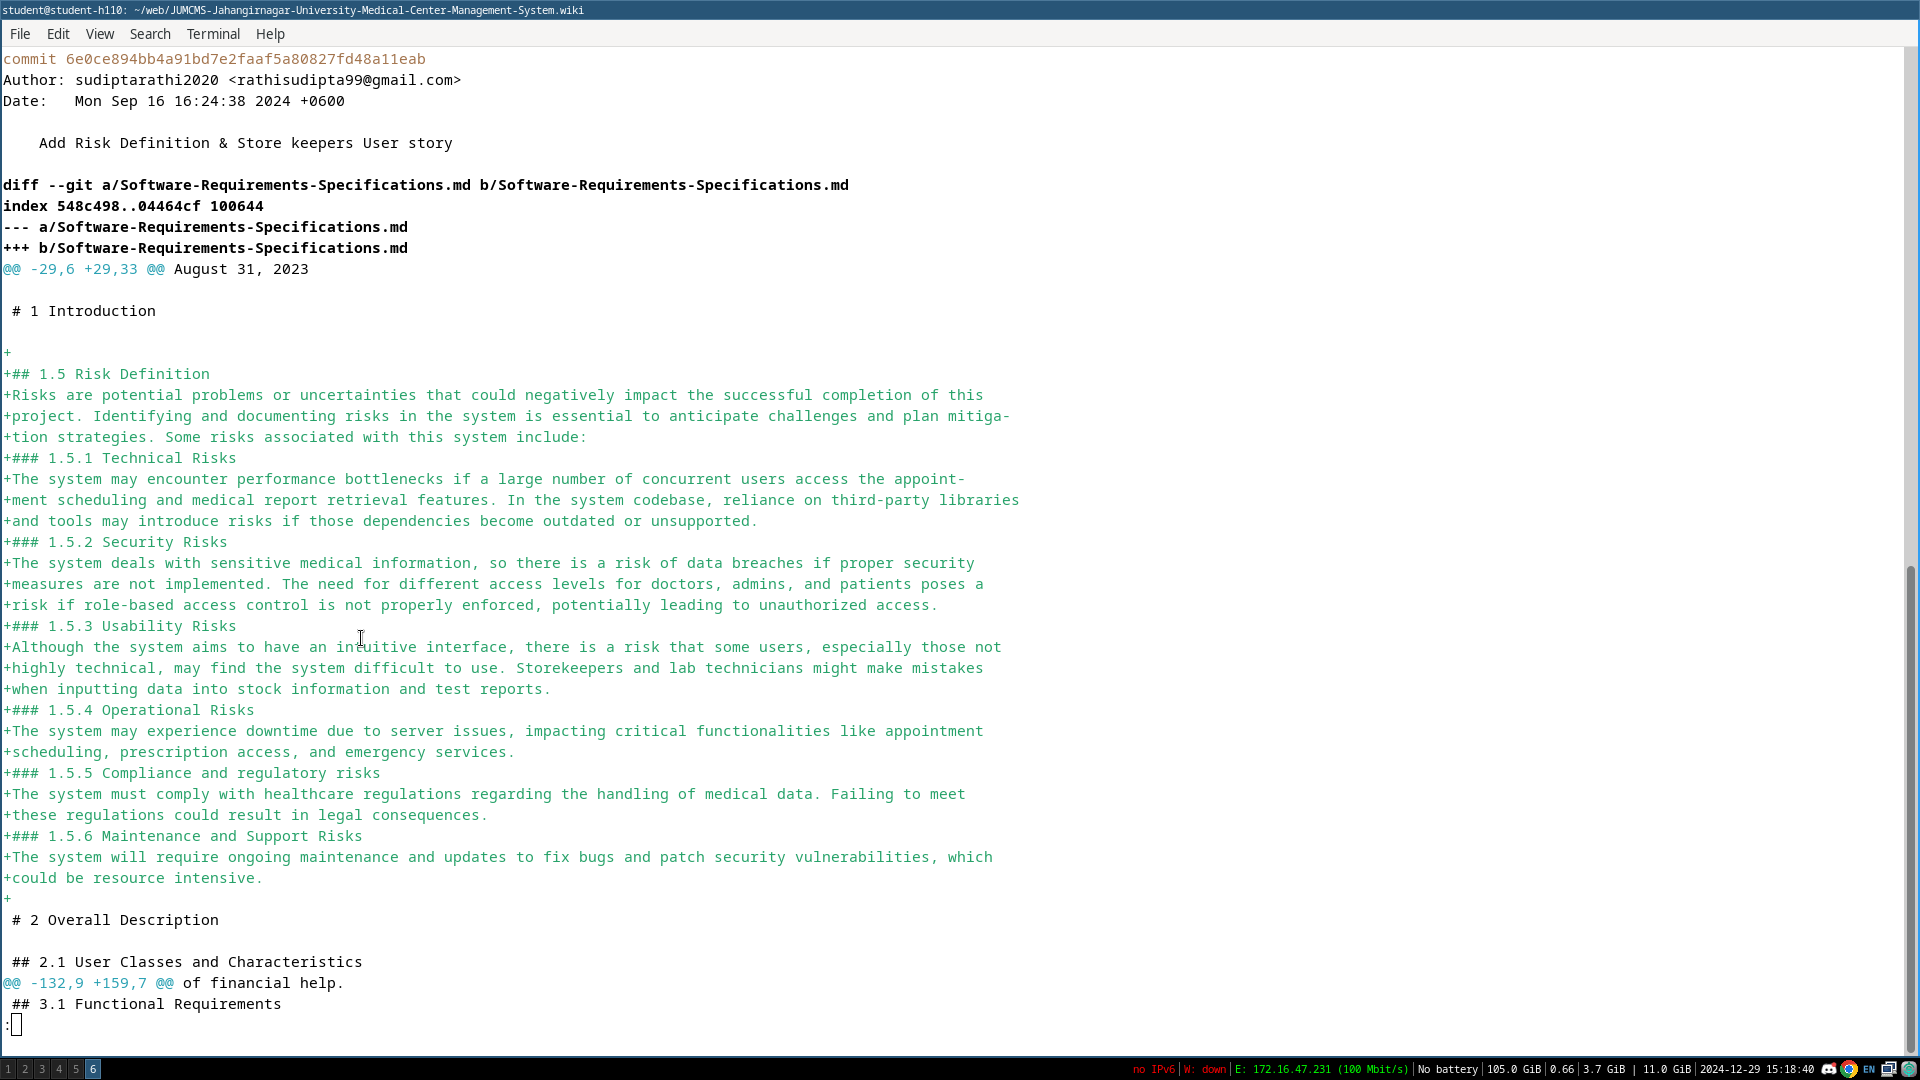
\includegraphics[width=0.8\textwidth]{images/git_srs.png}
    \caption{Git wiki commit for SRS}
    \label{fig:gitsrs}
\end{figure}

\subsection{Database Schema}
\begin{itemize}
    \item Designed the primary database schema
\end{itemize}
\begin{figure}[H]
    \centering
    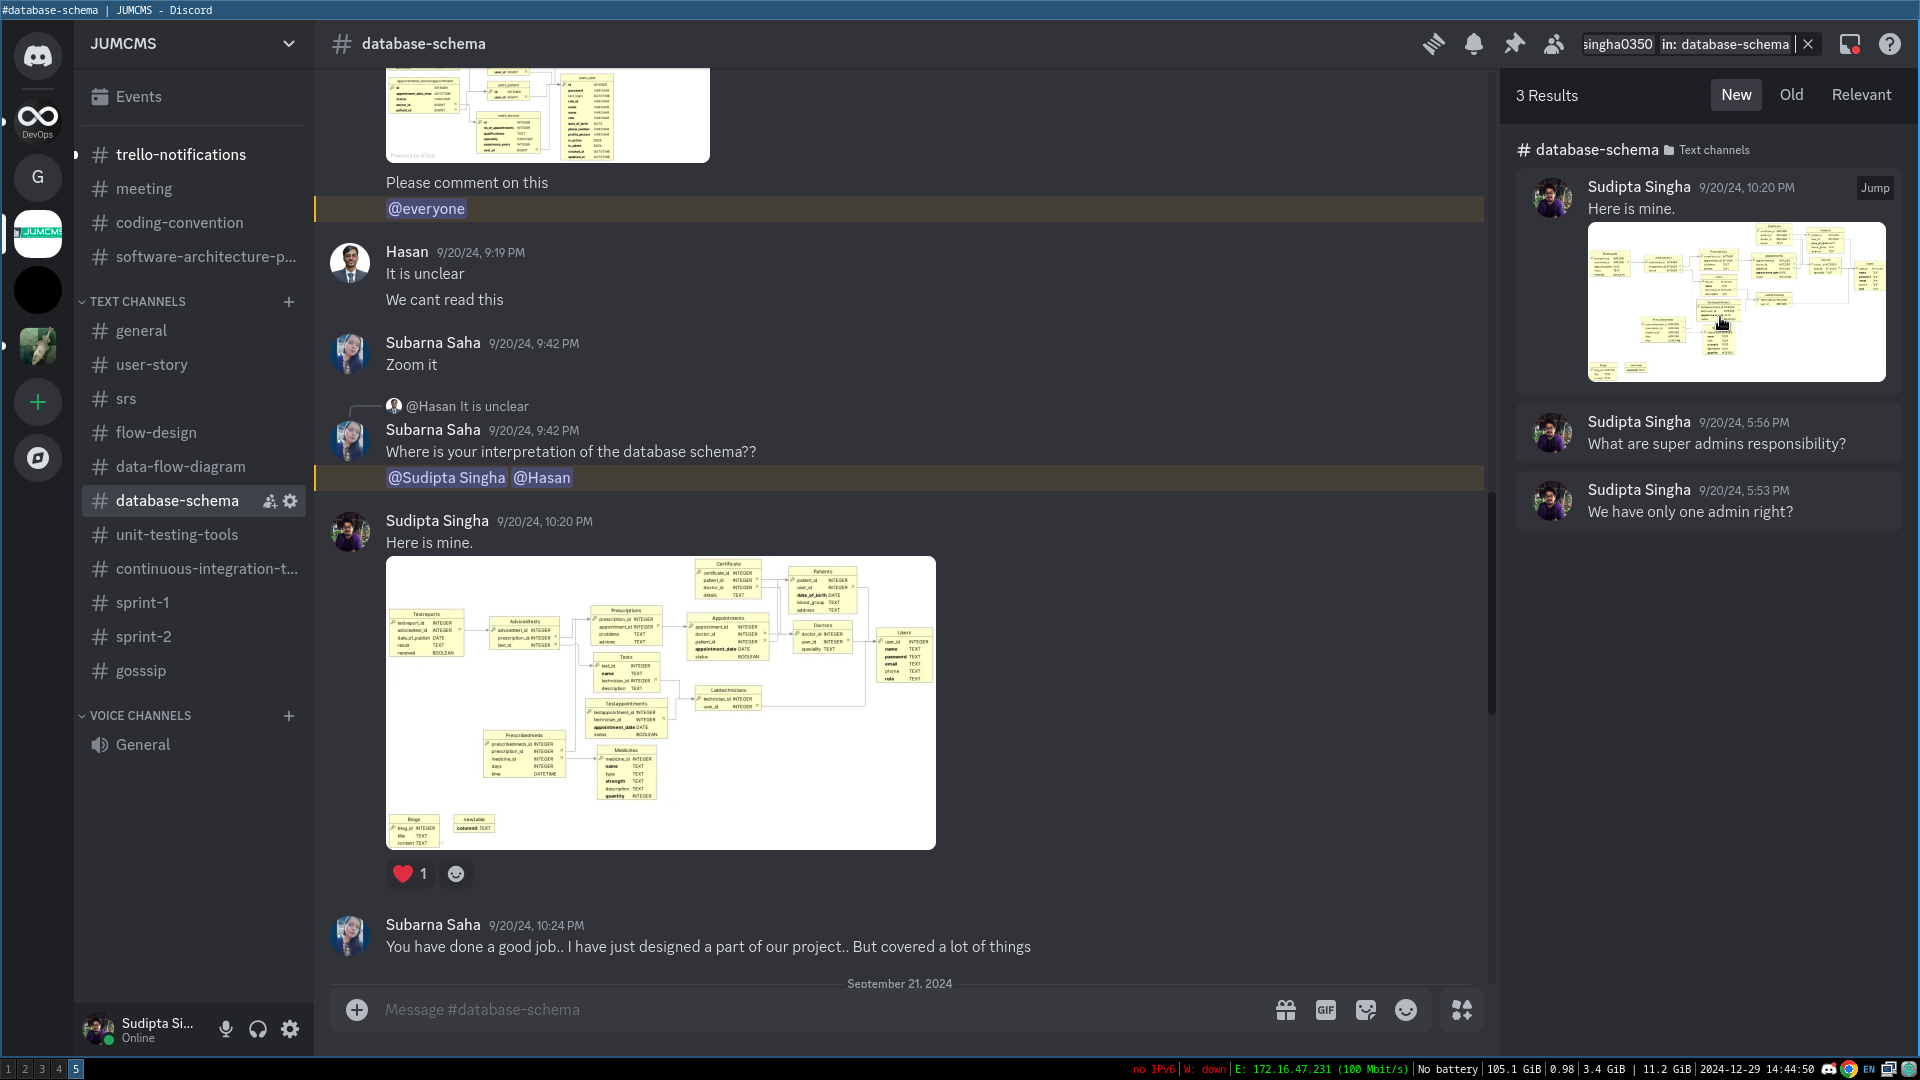
\includegraphics[width=0.8\textwidth]{images/discord_db.png}
    \caption{Discord conversation for DB design}
    \label{fig:discorddb}
\end{figure}
\begin{figure}[H]
    \centering
    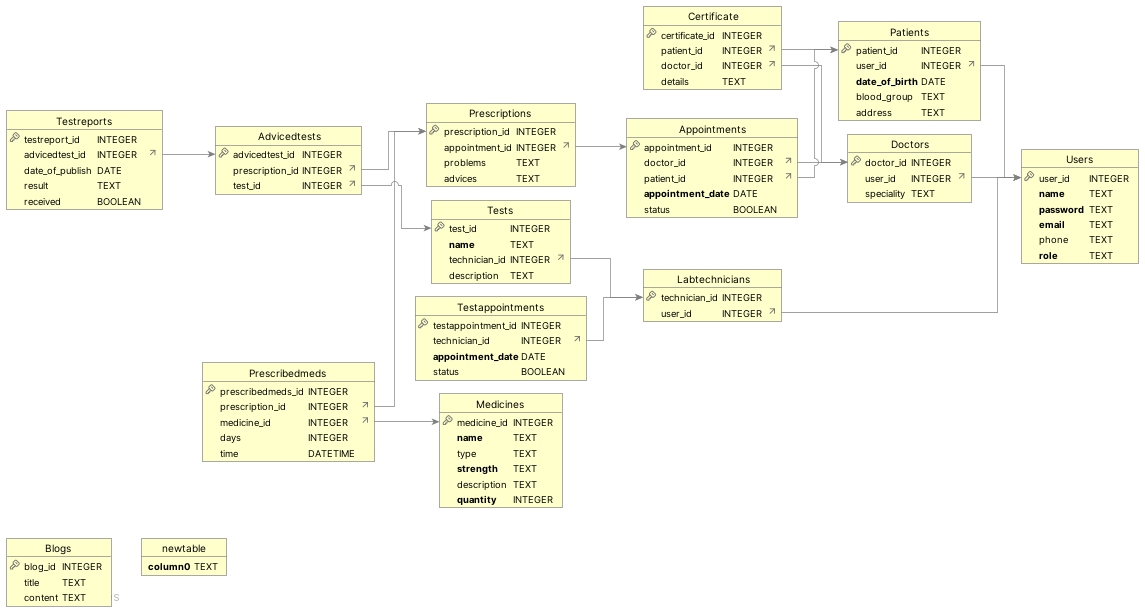
\includegraphics[width=0.8\textwidth]{images/dbschema.jpg}
    \caption{My designed database schema}
    \label{fig:db}
\end{figure}



\subsection{Software Architecture}
\begin{itemize}
    \item Wrote document about EBC design model which finally is not used in our project
\end{itemize}
\begin{figure}[H]
    \centering
    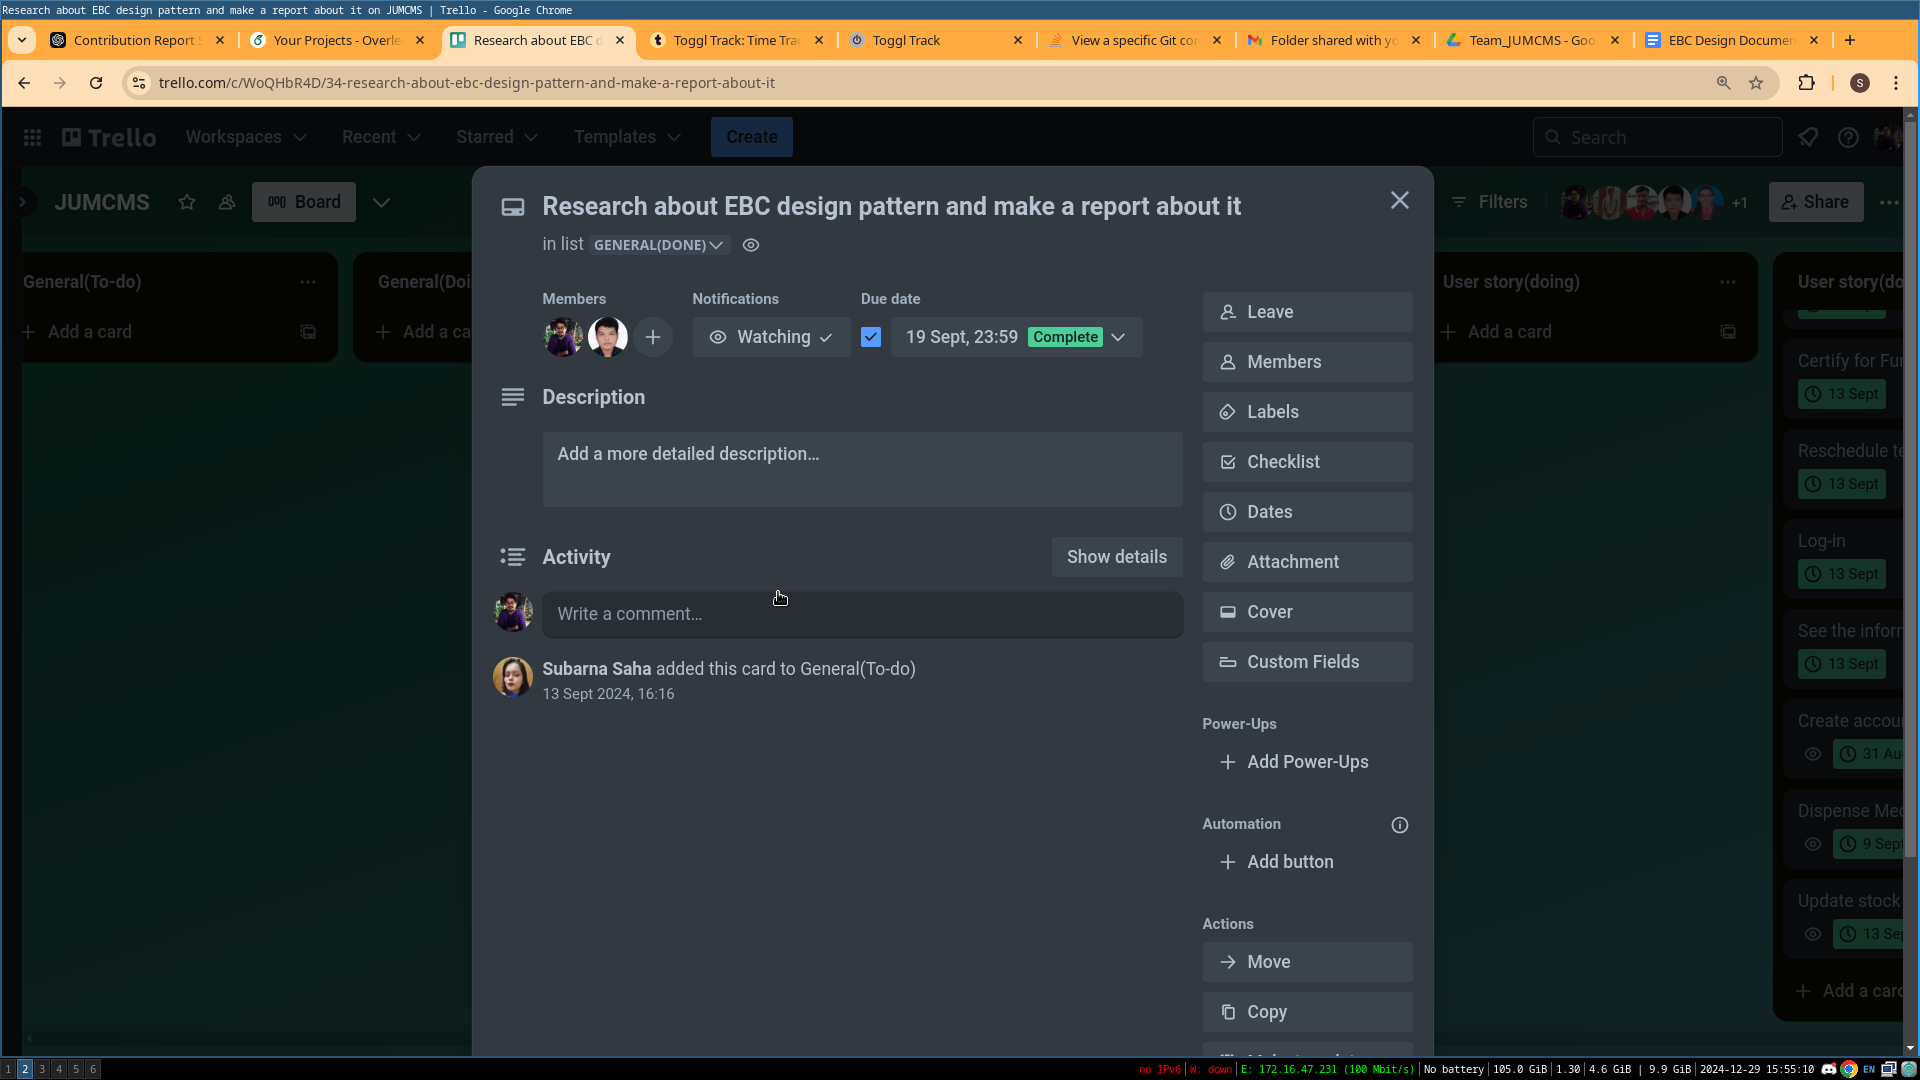
\includegraphics[width=0.8\textwidth]{images/trello_ebc.png}
    \caption{Trello work assignment for EBC design}
    \label{fig:ebcdesignreport}
\end{figure}


\begin{figure}[H]
    \centering
    
\includegraphics[width=0.8\textwidth]{images/ebc_report.png}
    \caption{EBC Report}
    \label{fig:ebc}
\end{figure}


\subsection{Coding Convention}
\begin{itemize}
    \item Wrote report about Python coding convention.
\end{itemize}

\begin{figure}[H]
    \centering
    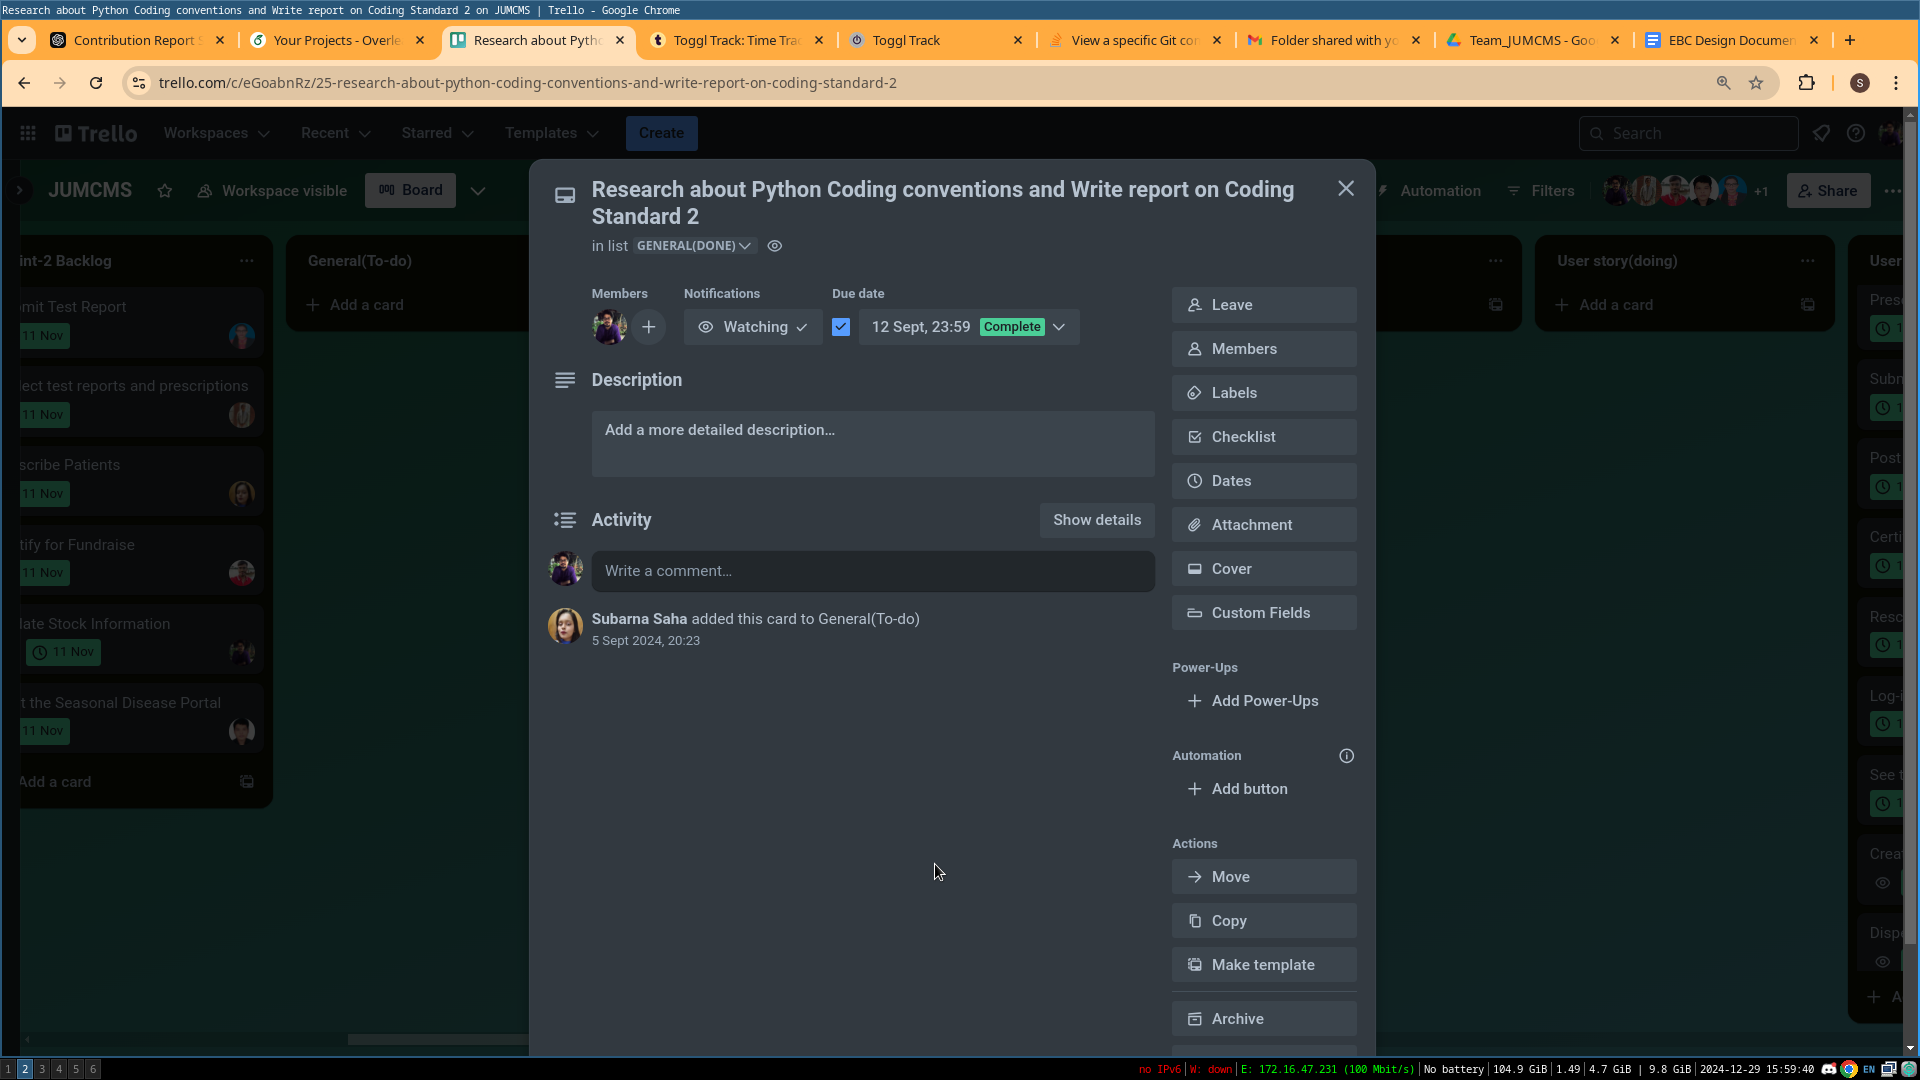
\includegraphics[width=0.8\textwidth]{images/trello_coding_convention.png}
    \caption{Trello work assignment for coding convenation}
    \label{fig:trellocodingconventionreport}
\end{figure}


\begin{figure}[H]
    \centering
    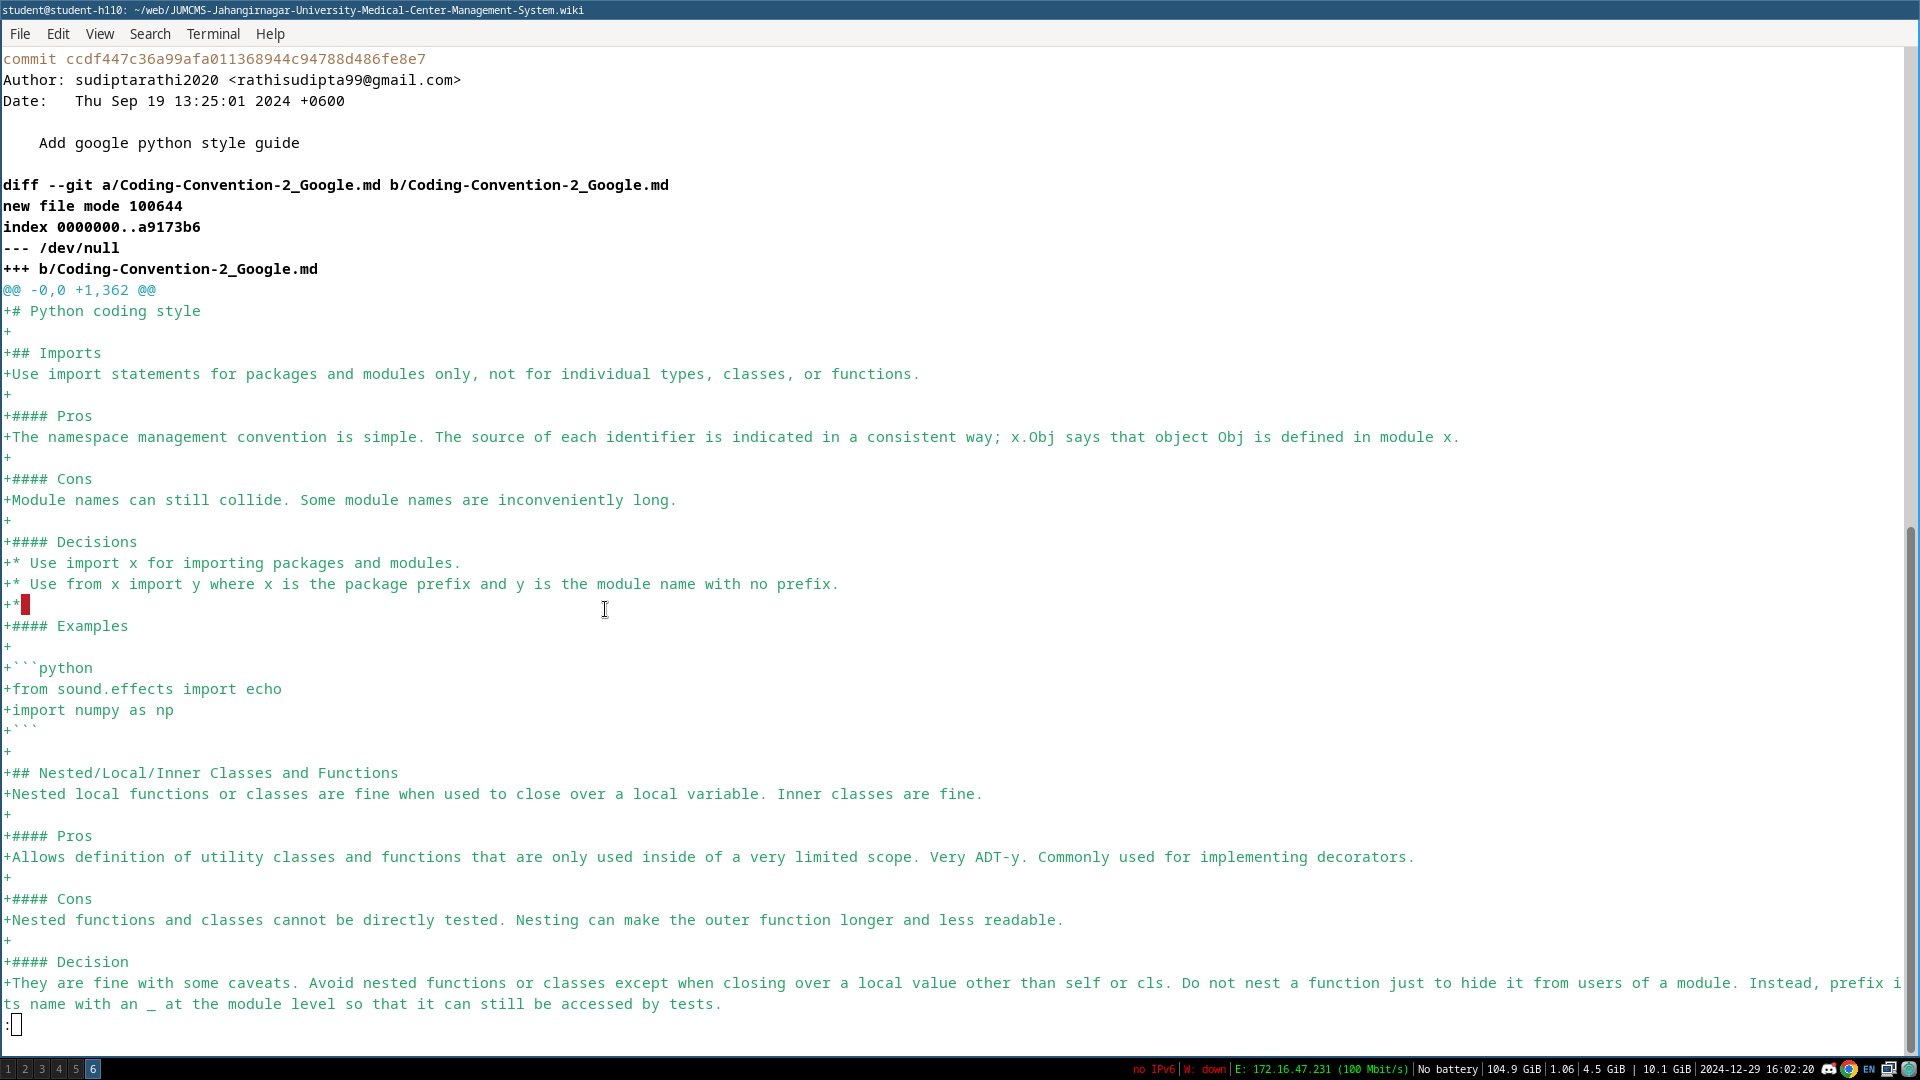
\includegraphics[width=0.8\textwidth]{images/git_coding_convention.png}
    \caption{Git log of coding convention report}
    \label{fig:gitcodingconvention}
\end{figure}


\subsection{CICD tool research}
\begin{itemize}
    \item Researched about Travis CI cicd tool
    \item Researched about github actions cicd tool
\end{itemize}

\begin{figure}[H]
    \centering
    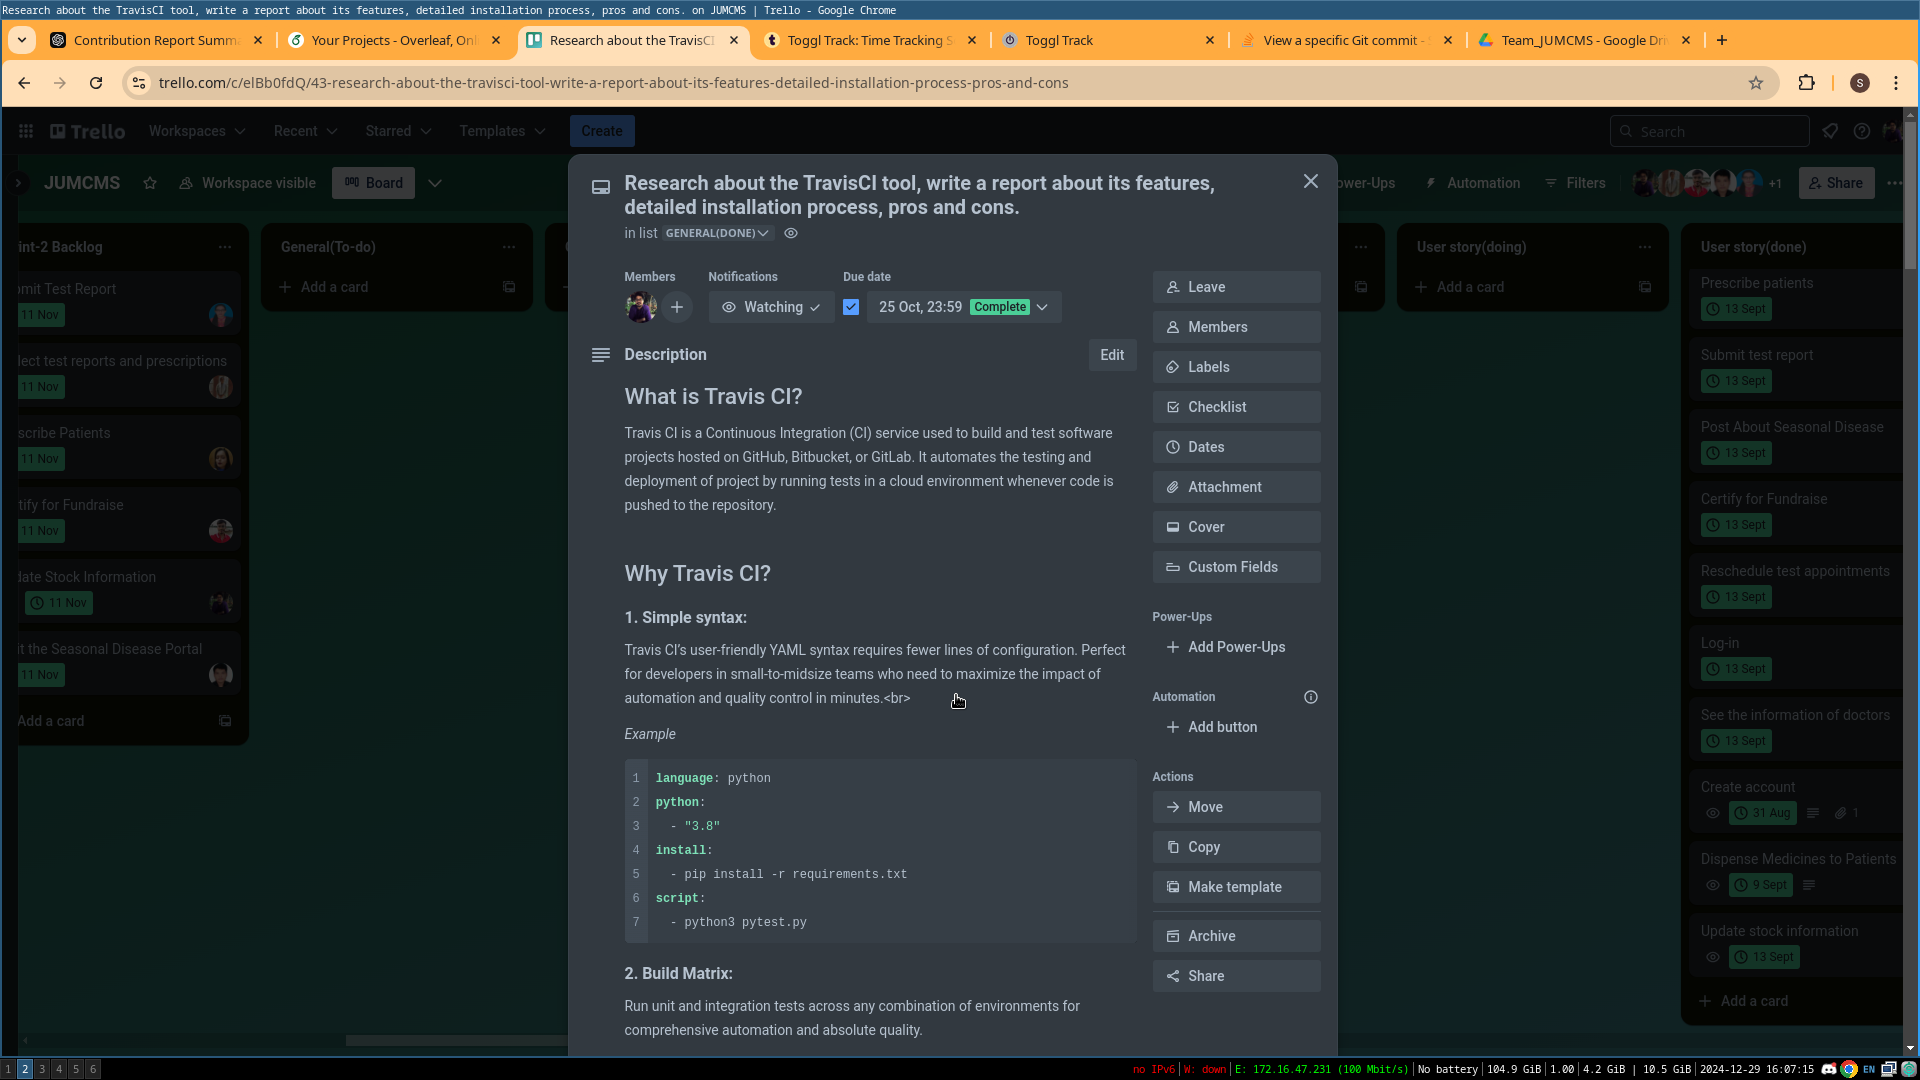
\includegraphics[width=0.8\textwidth]{images/trello_cicd.png}
    \caption{Trello work assignment for continous integration and continous development}
    \label{fig:trellocicd}
\end{figure}


\begin{figure}[H]
    \centering
    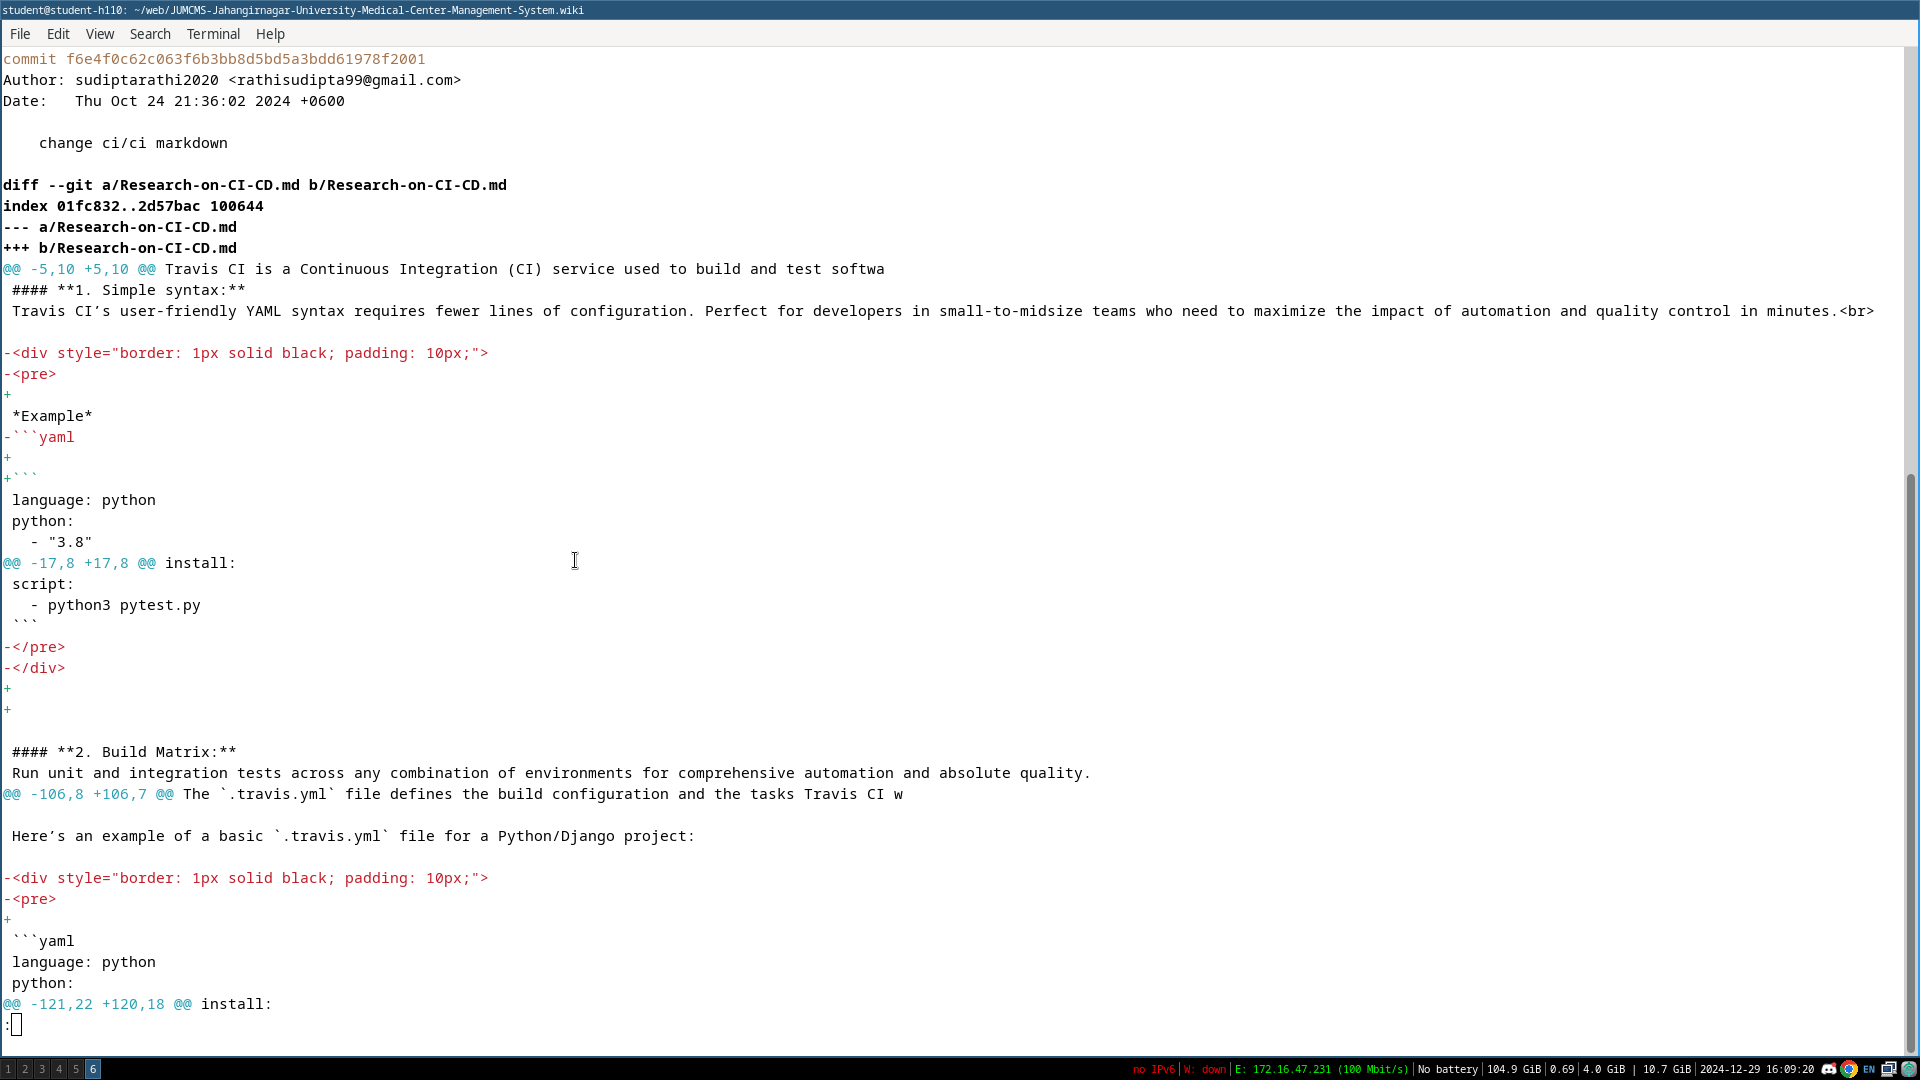
\includegraphics[width=0.8\textwidth]{images/git_cicd_travis.png}
    \caption{Git log of Travis CI report}
    \label{fig:gitcicd}
\end{figure}


\begin{figure}[H]
    \centering
    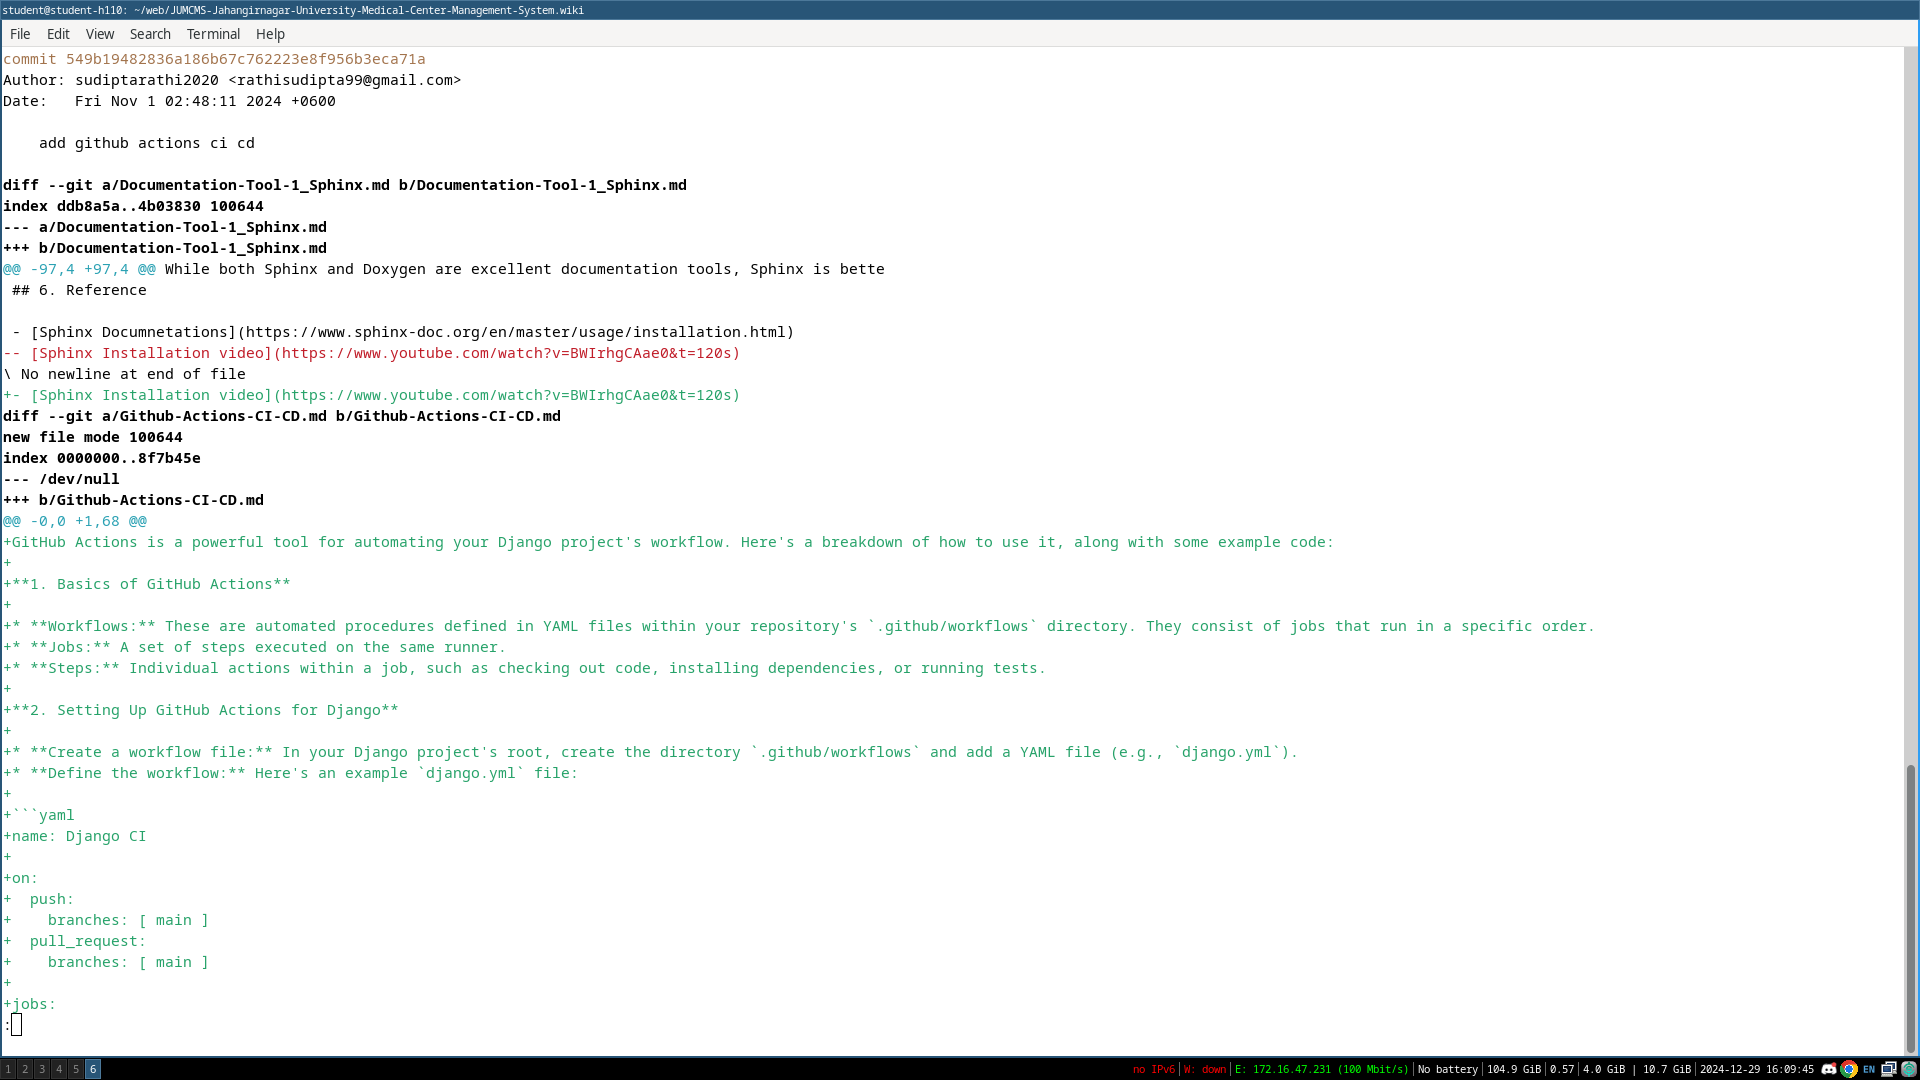
\includegraphics[width=0.8\textwidth]{images/git_cicd_github.png}
    \caption{Git log of github actions report}
    \label{fig:githubactins}
\end{figure}


\subsection{Sprint 1}
In sprint 1 , I was assigned various features.
\begin{itemize}
    \item Create Account
    \item Dispense Medicines to Patient
    \item Help others in setting up django project
\end{itemize}
\begin{figure}[H]
    \centering
    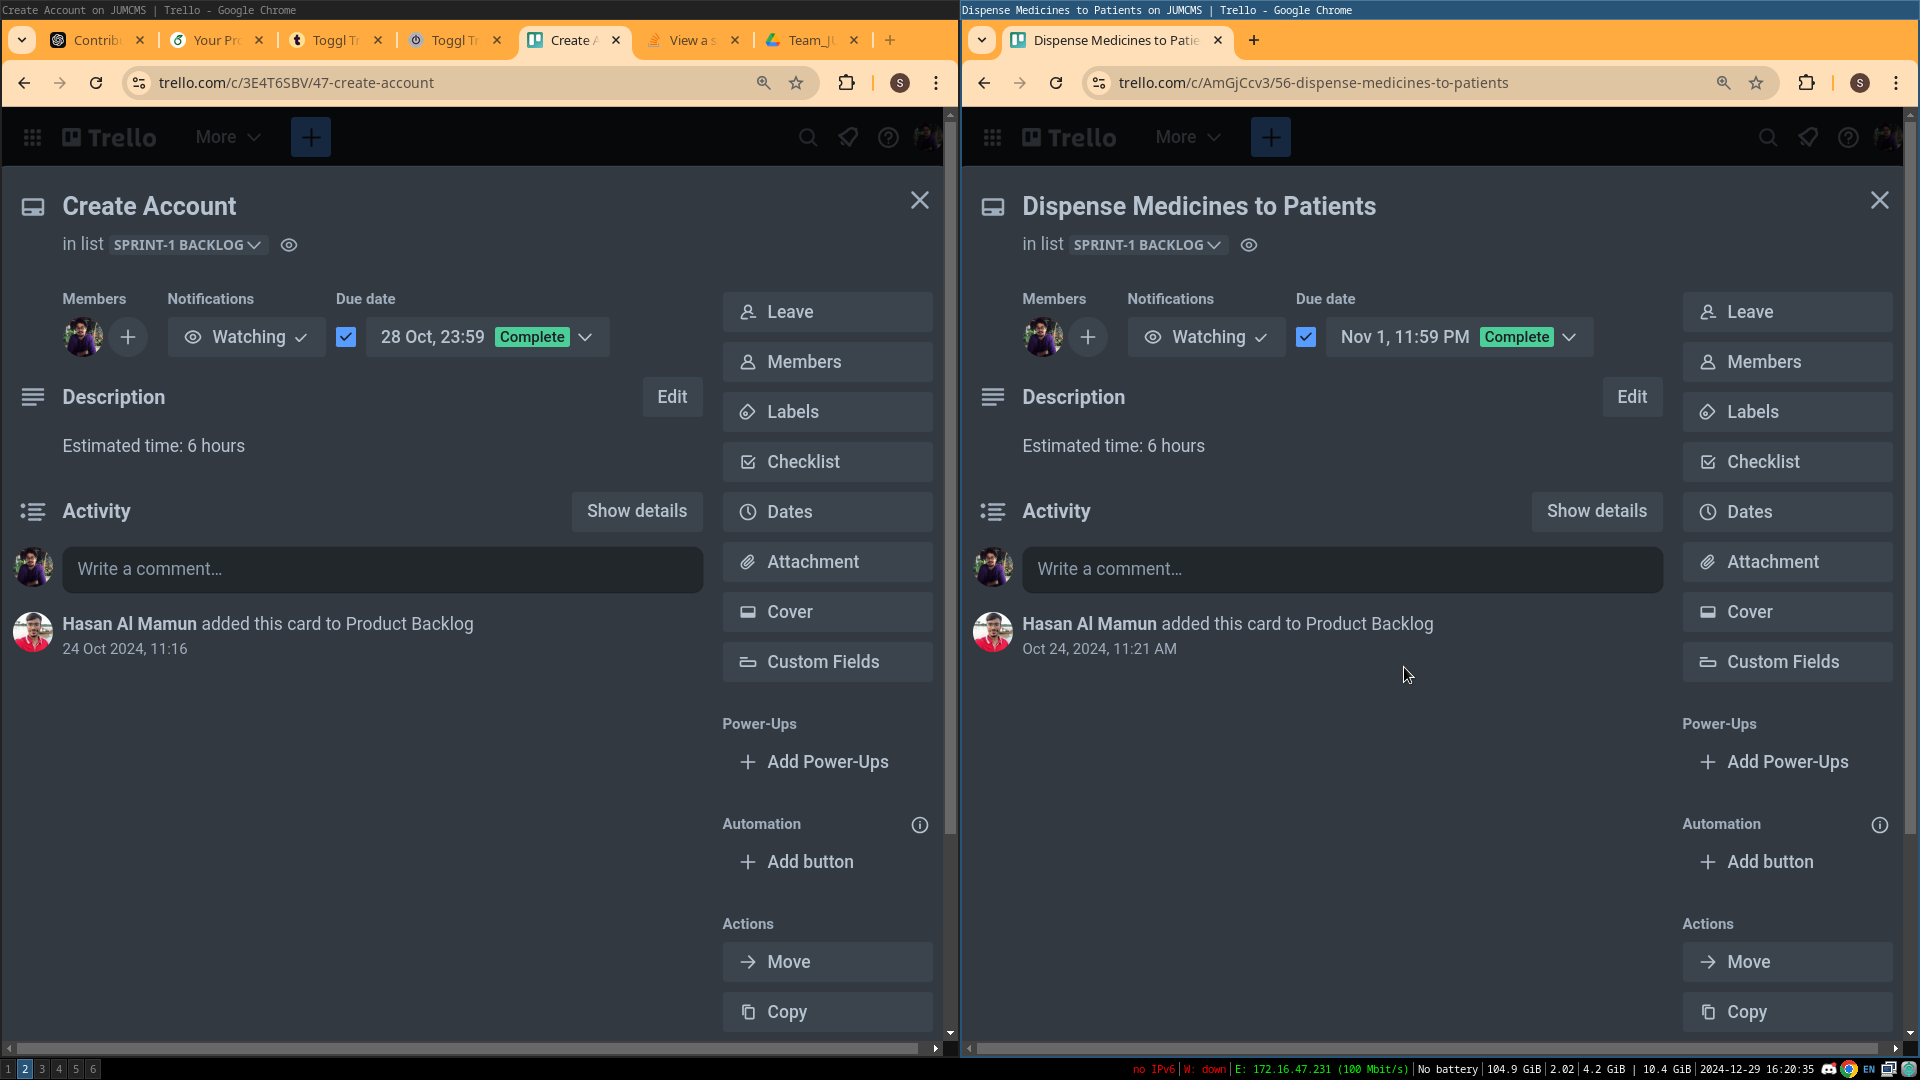
\includegraphics[width=0.8\textwidth]{images/trello_sprint1.png}
    \caption{Trello for Sprint 1}
    \label{fig:trellosprint1}
\end{figure}


\begin{figure}[H]
    \centering
    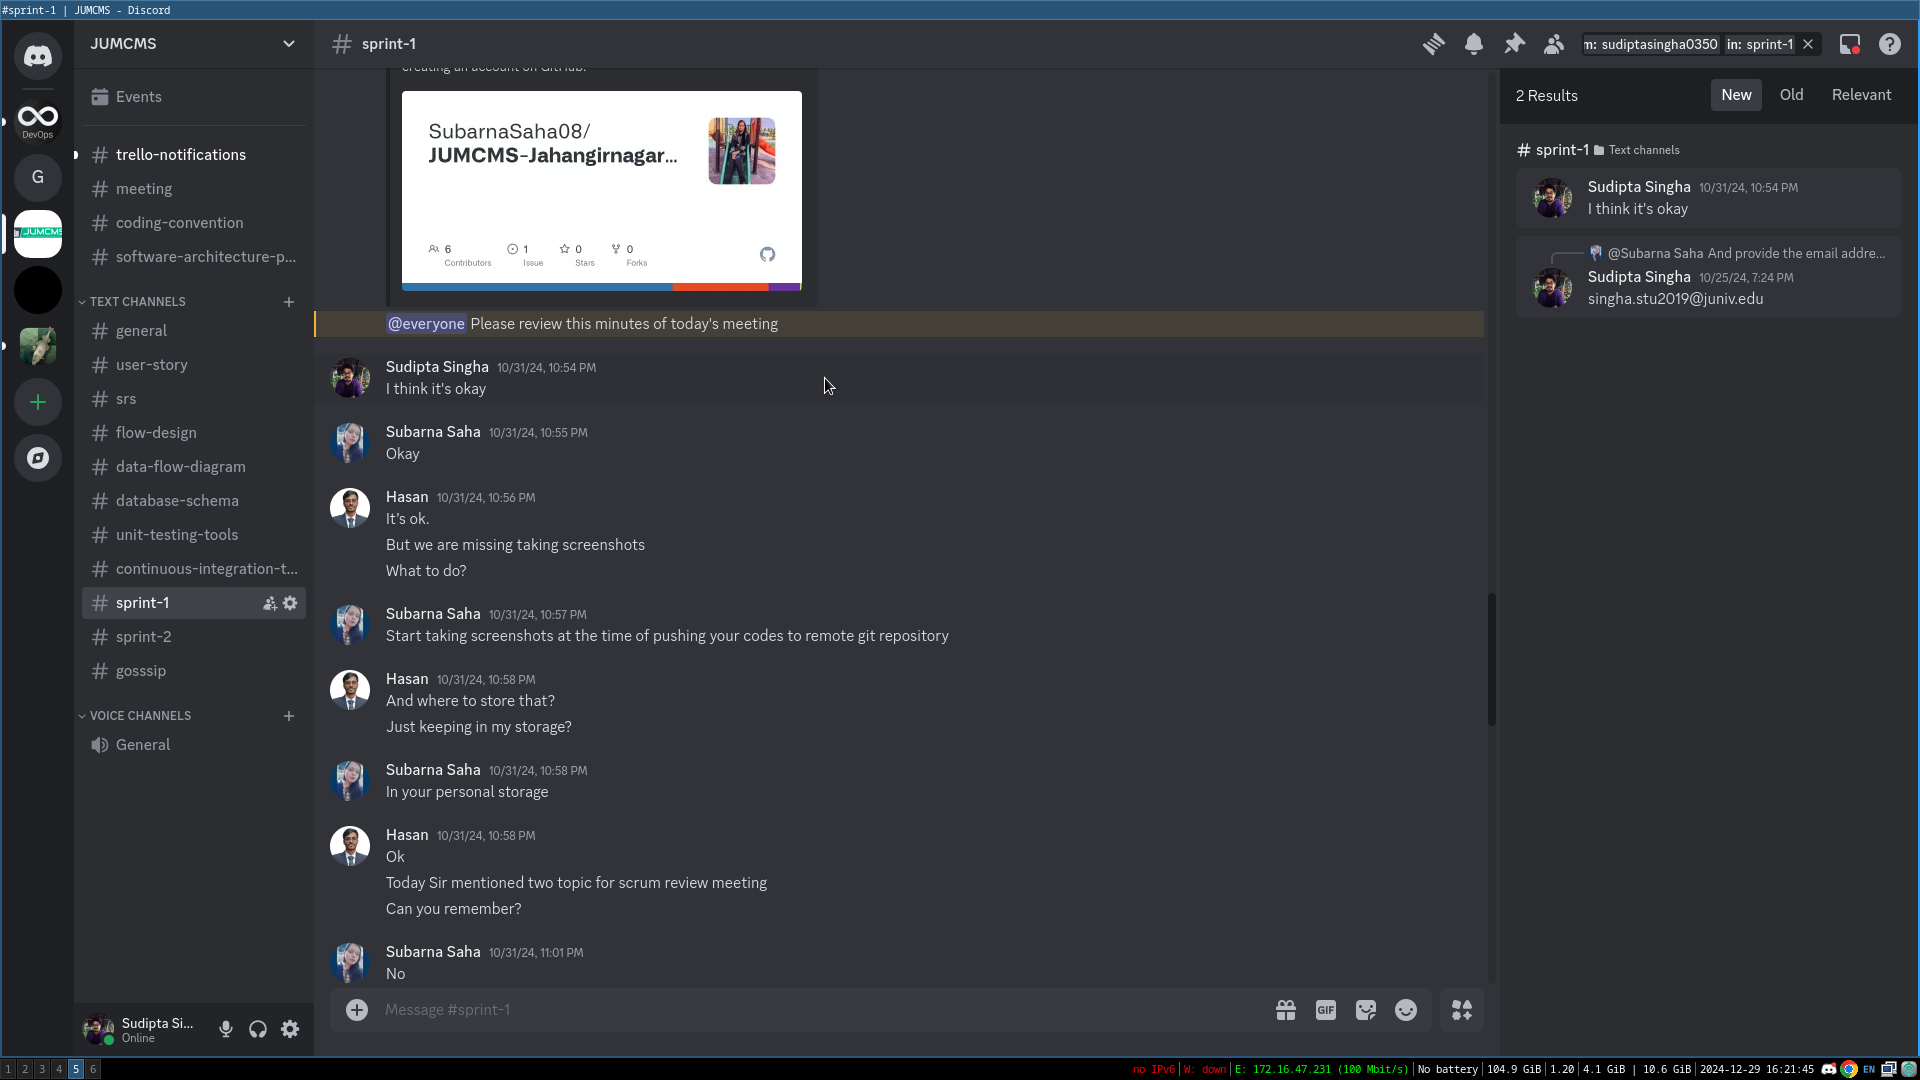
\includegraphics[width=0.8\textwidth]{images/discord_sprint1.png}
    \caption{Discord for Sprint 1}
    \label{fig:discordsprint1}
\end{figure}


\begin{figure}[H]
    \centering
    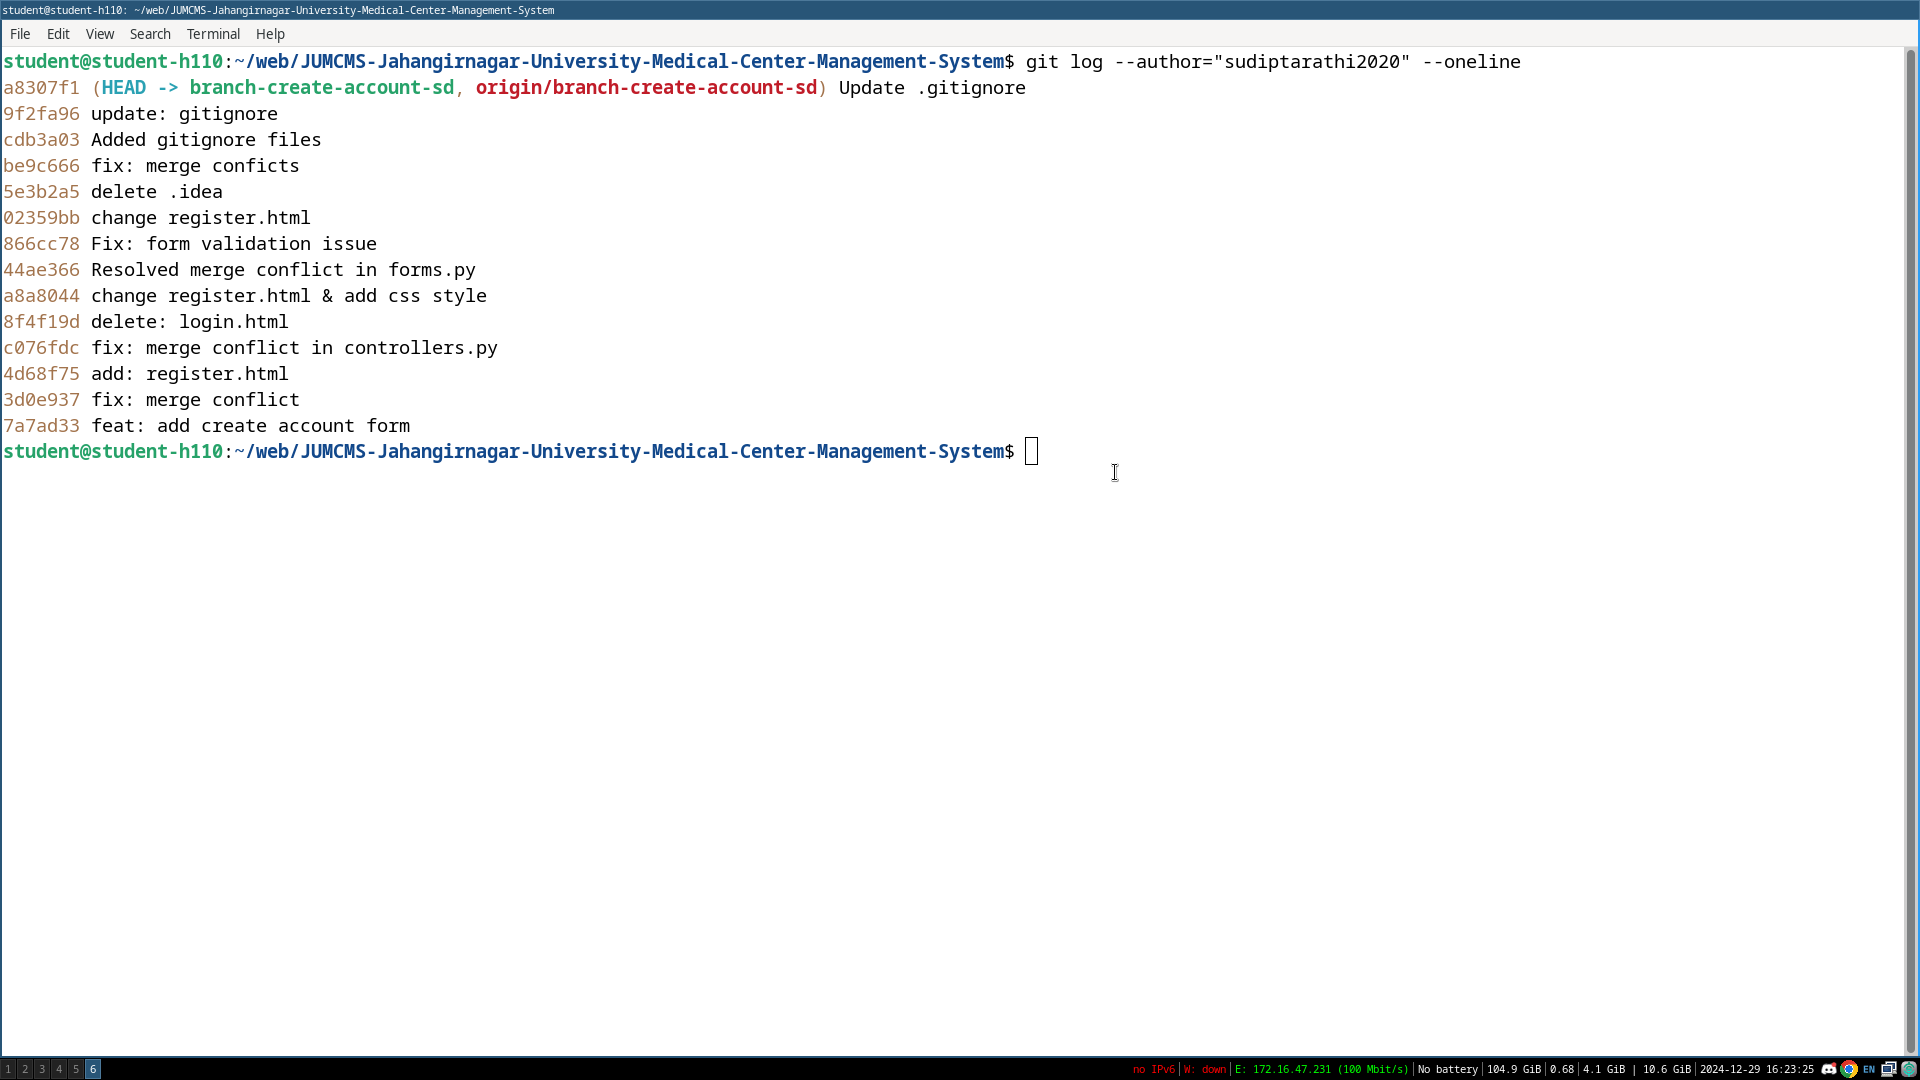
\includegraphics[width=0.8\textwidth]{images/git_sprint1.png}
    \caption{Git log for Create Account feature}
    \label{fig:gitlogcreateaccount}
\end{figure}


\begin{figure}[H]
    \centering
    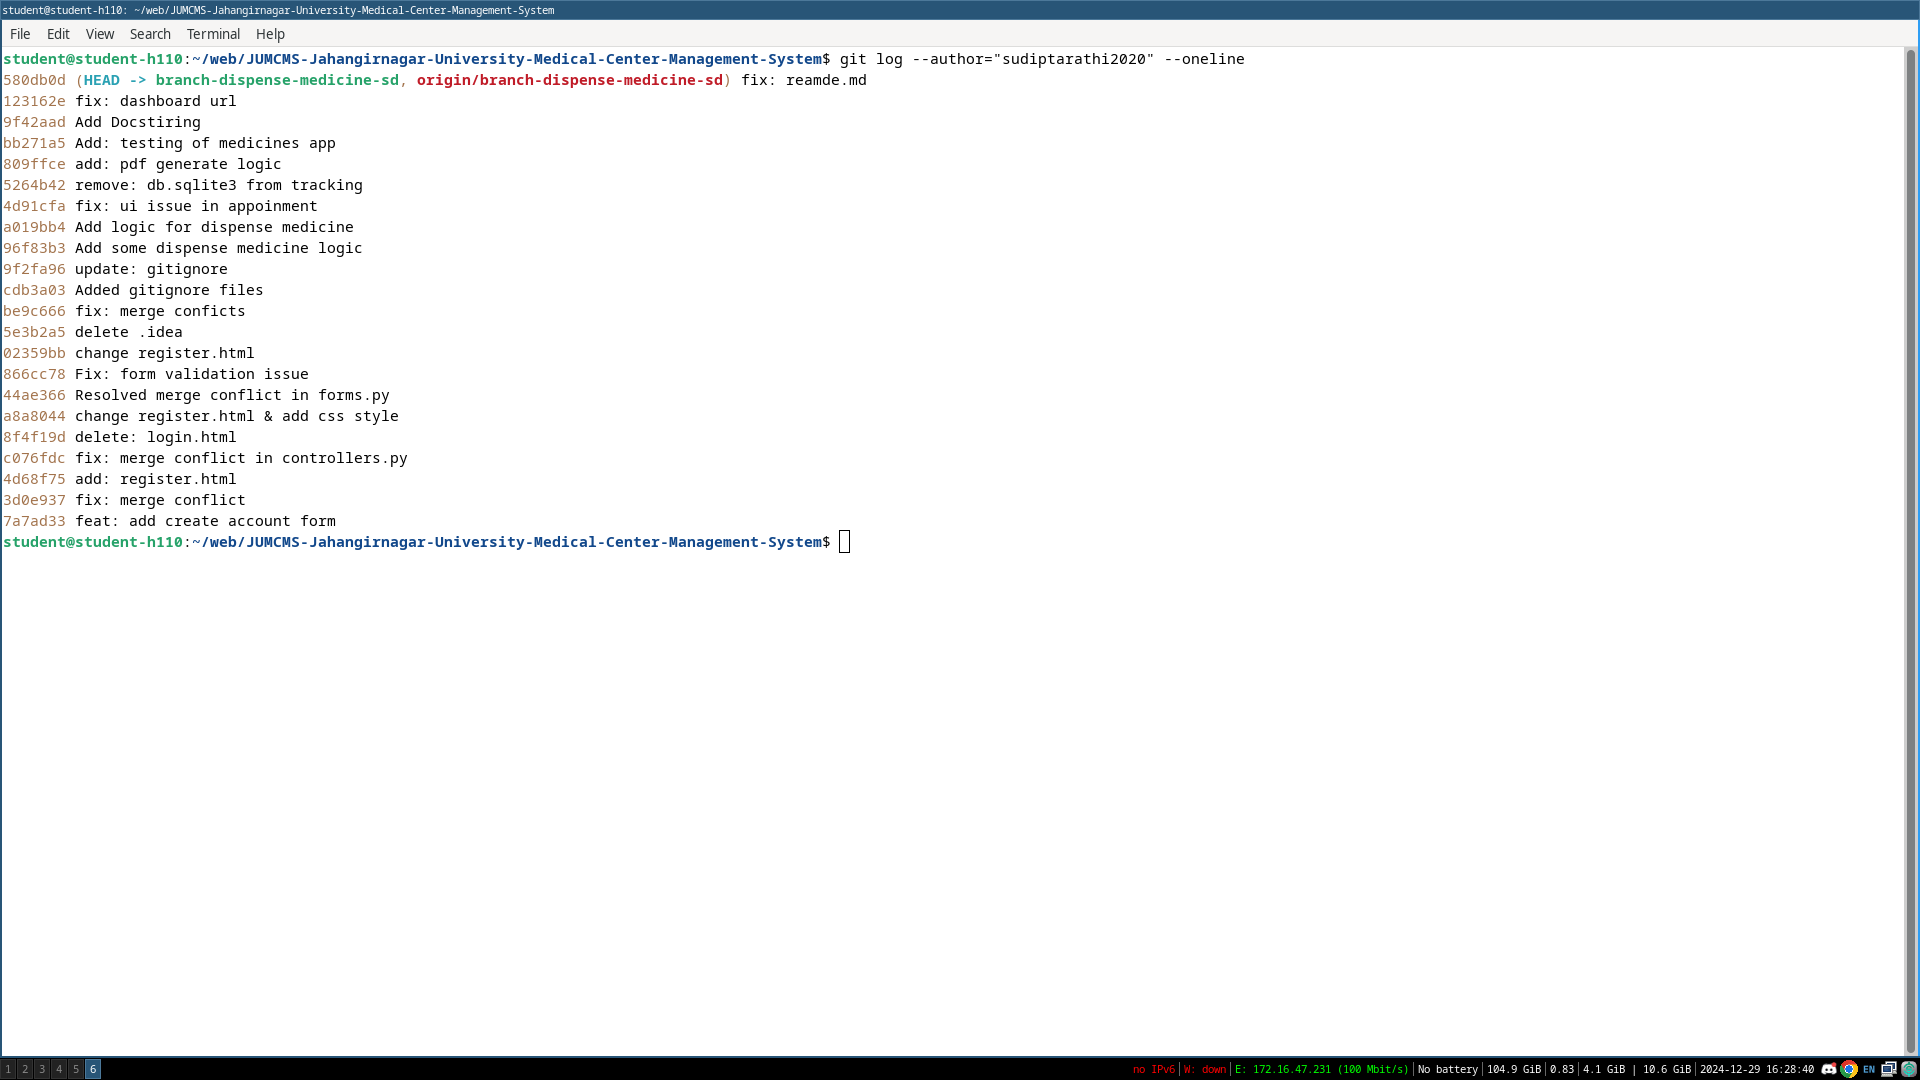
\includegraphics[width=0.8\textwidth]{images/git_sprint1_1.png}
    \caption{Git log for Dispense medicines feature}
    \label{fig:gitlogdispensemedicine}
\end{figure}


\begin{figure}[H]
    \centering
    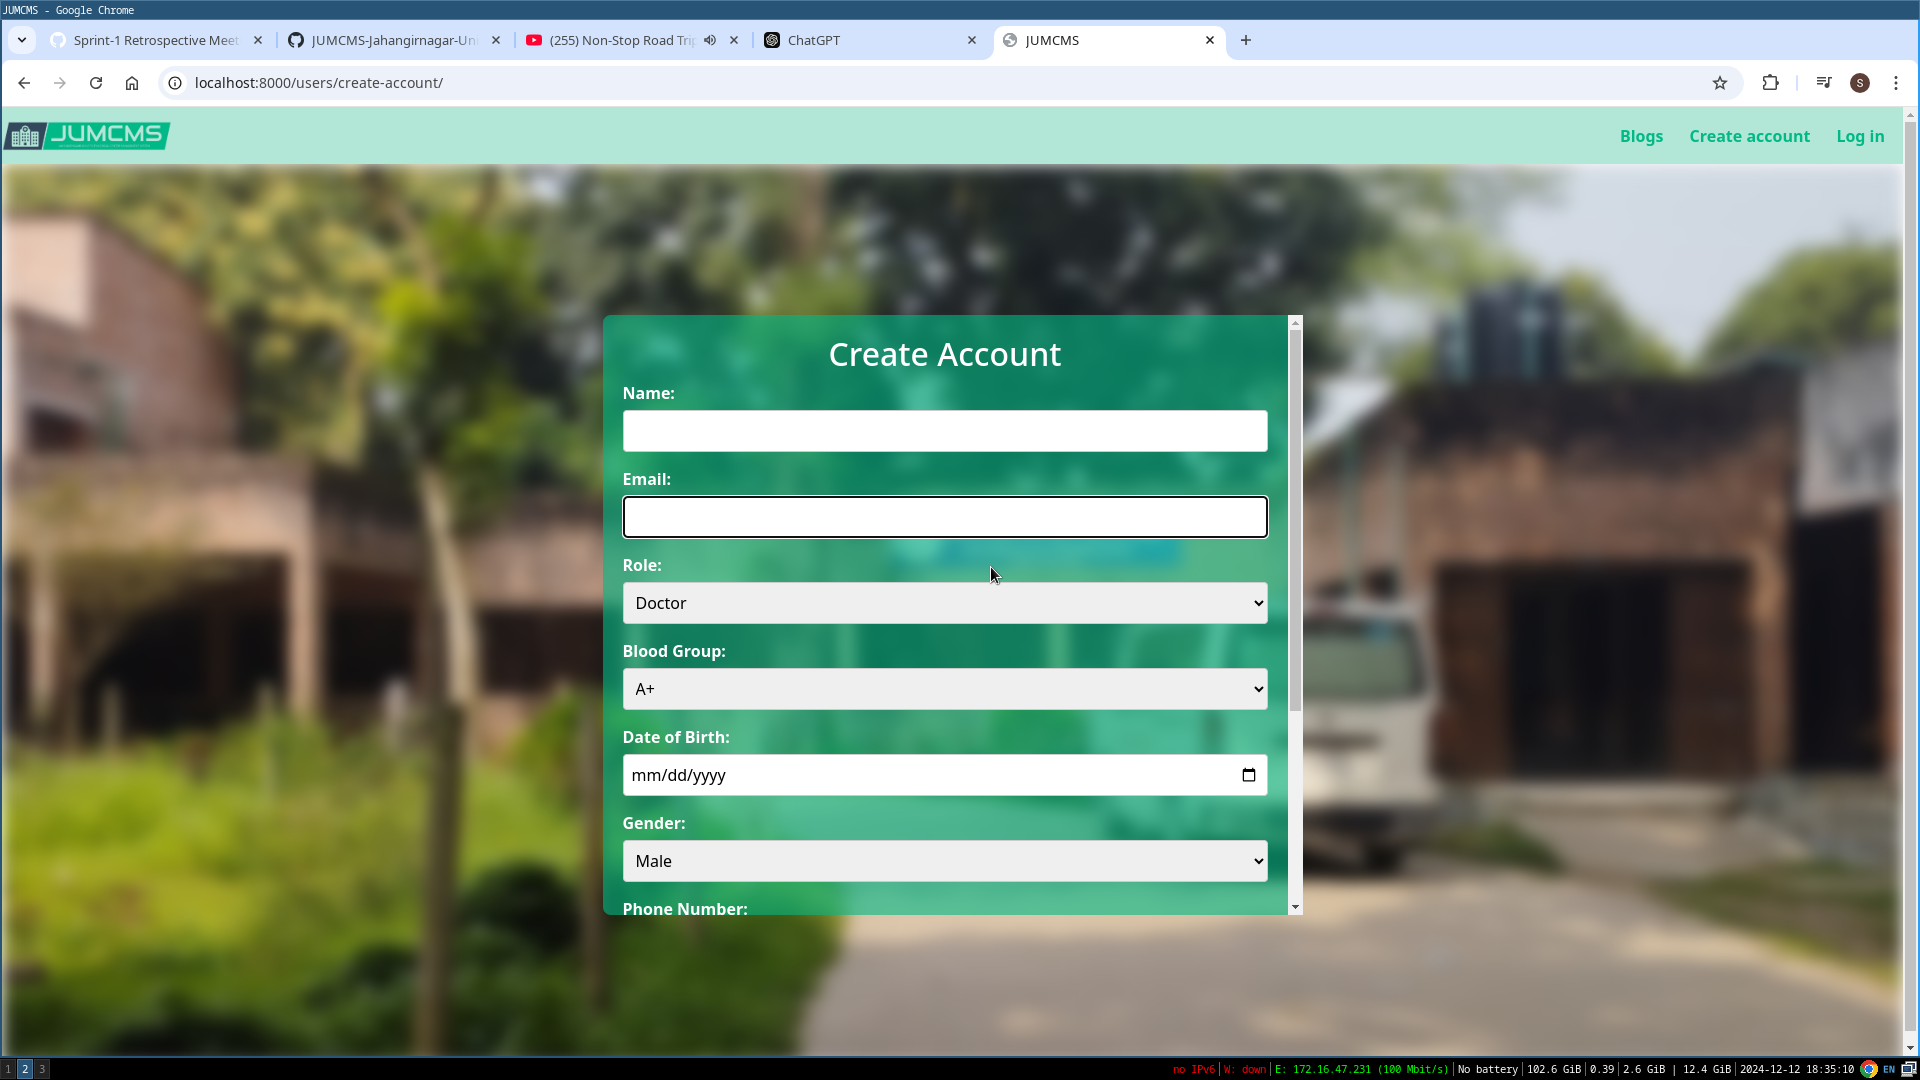
\includegraphics[width=0.8\textwidth]{images/spr1output2.png}
    \caption{Output of Create account sprint}
    \label{fig:sp1out1}
\end{figure}


\begin{figure}[H]
    \centering
    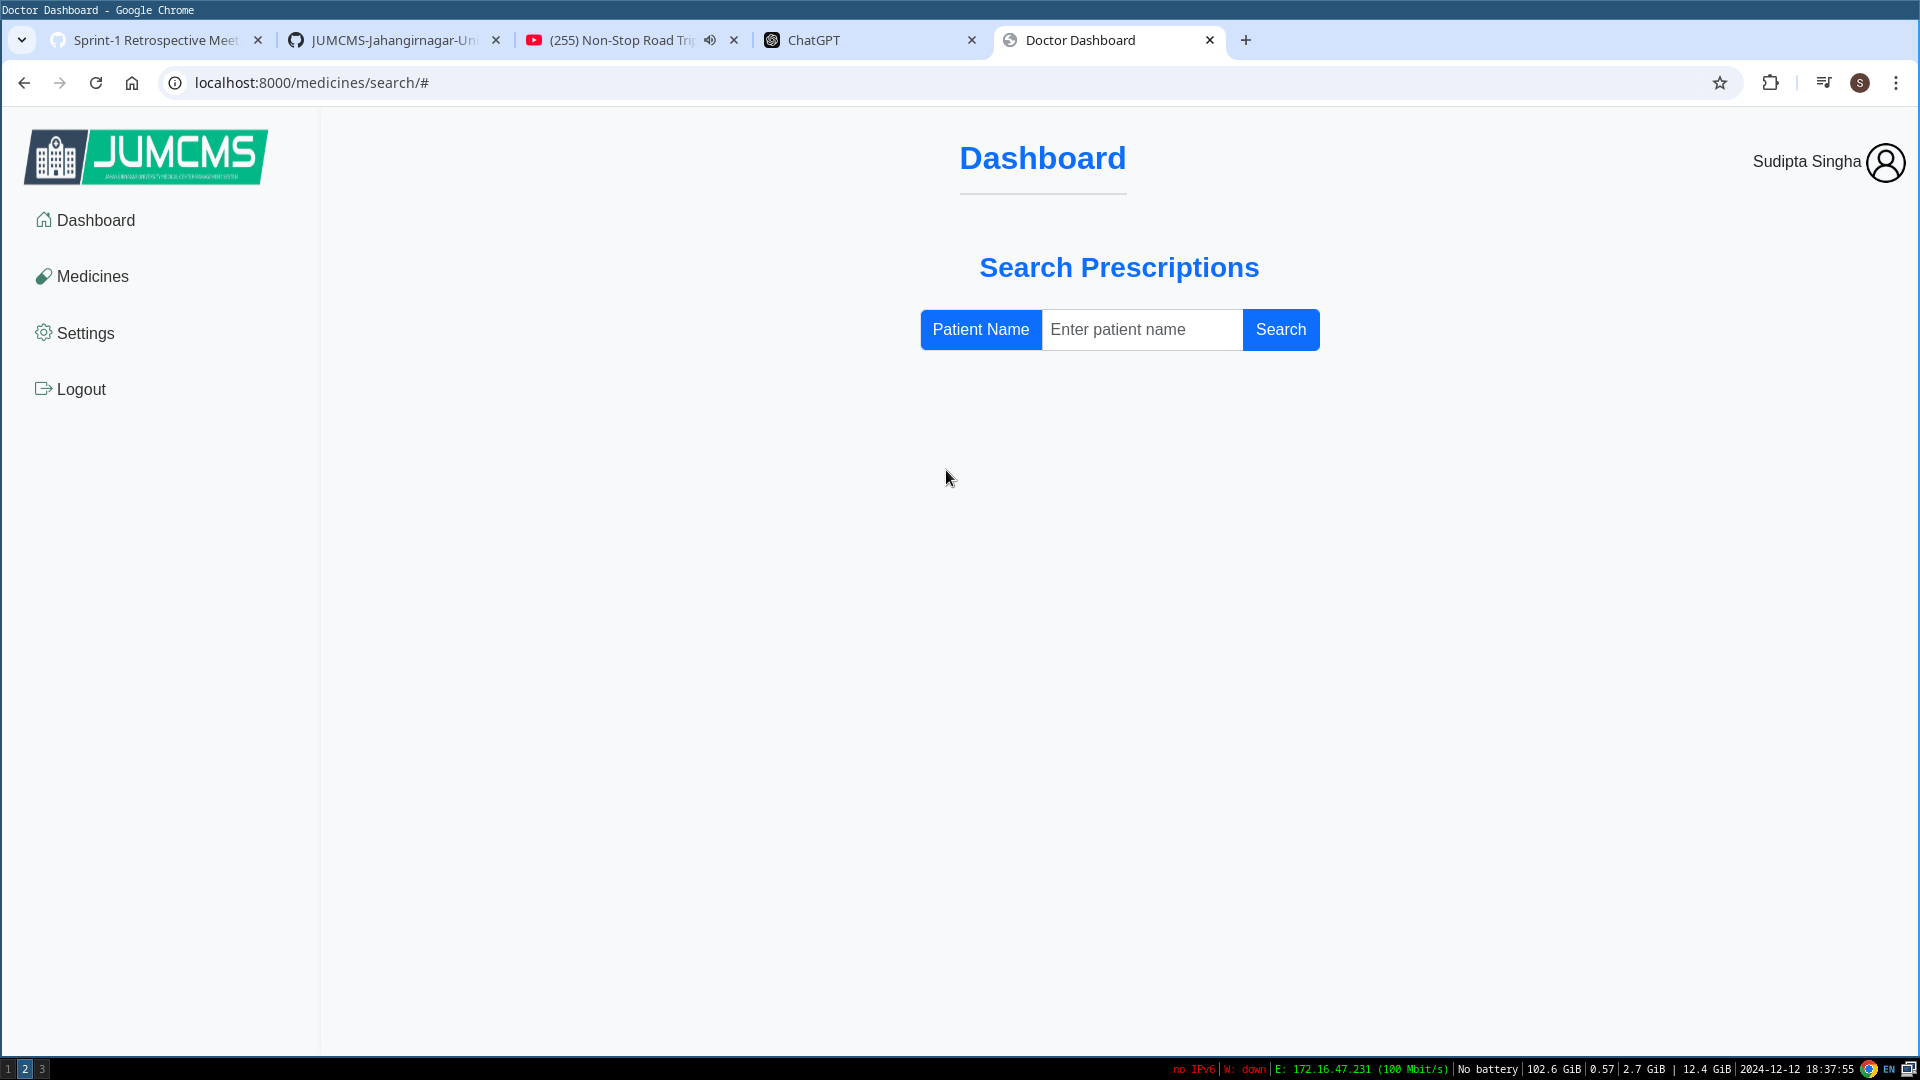
\includegraphics[width=0.8\textwidth]{images/spr1output3.png}
    \caption{Output of Dispense Medicines to patient}
    \label{fig:sp1out2}
\end{figure}

\begin{figure}[H]
    \centering
    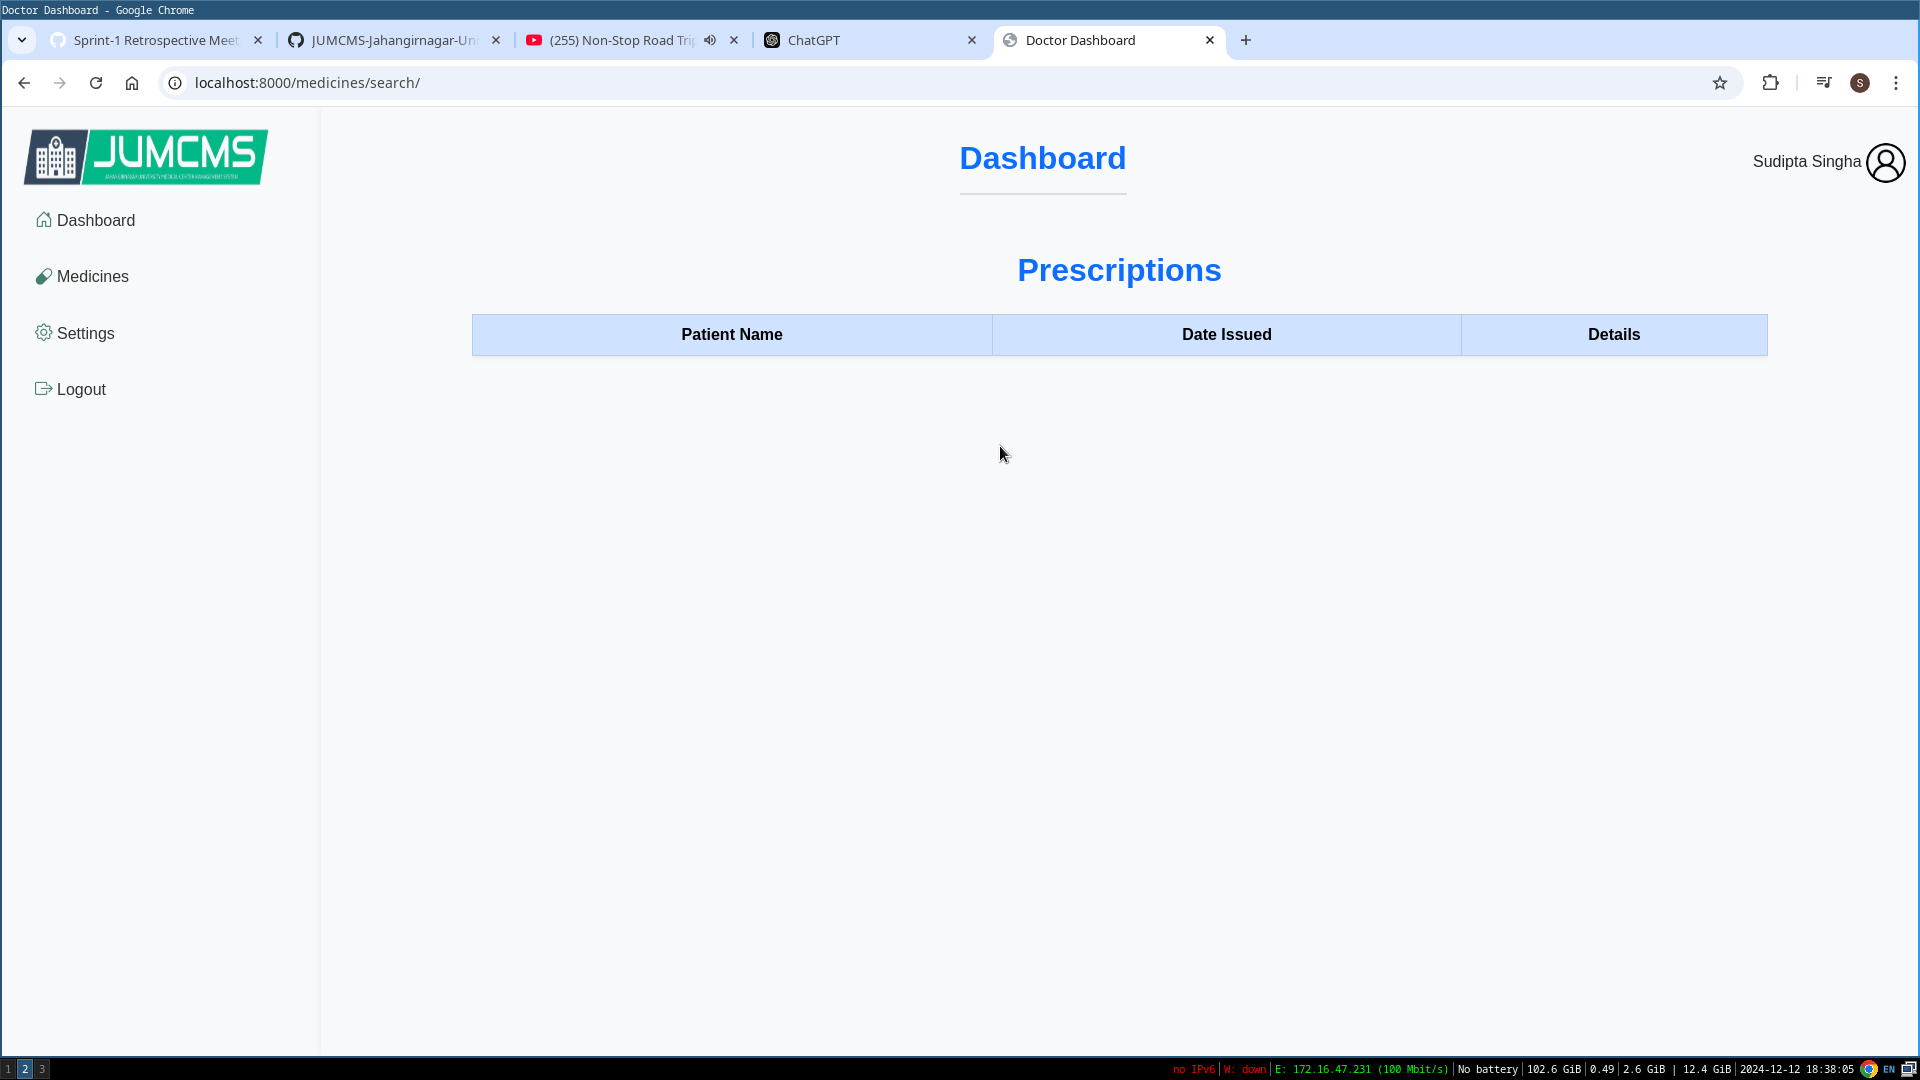
\includegraphics[width=0.8\textwidth]{images/spr1output4.png}
    \caption{Output of Dispense Medicines to patient}
    \label{fig:sp1out3}
\end{figure}



\subsection{Sprint 2}
In sprint 2 , I was assigned various features.
\begin{itemize}
    \item Create Account
\end{itemize}

\begin{figure}[H]
    \centering
    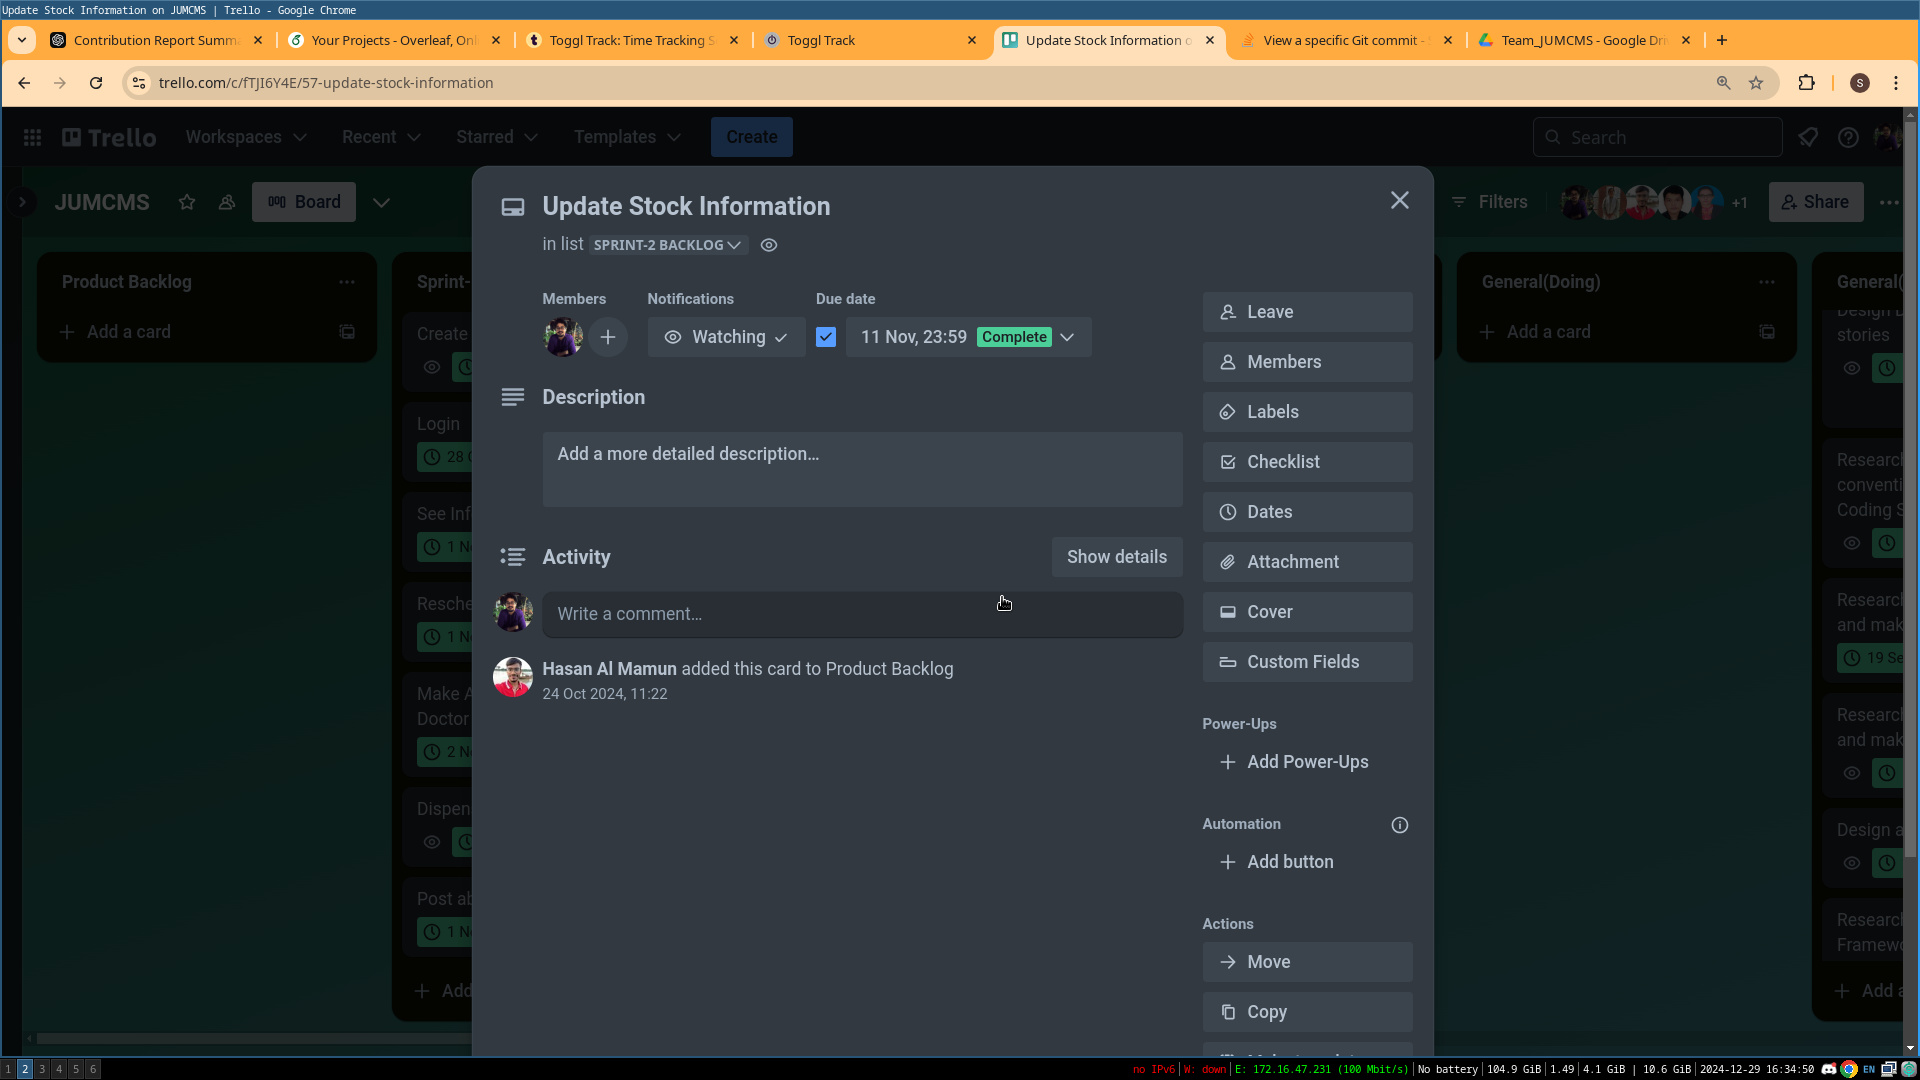
\includegraphics[width=0.8\textwidth]{images/trello_sprint2.png}
    \caption{Trello for Sprint 2}
    \label{fig:trellosprint2}
\end{figure}


\begin{figure}[H]
    \centering
    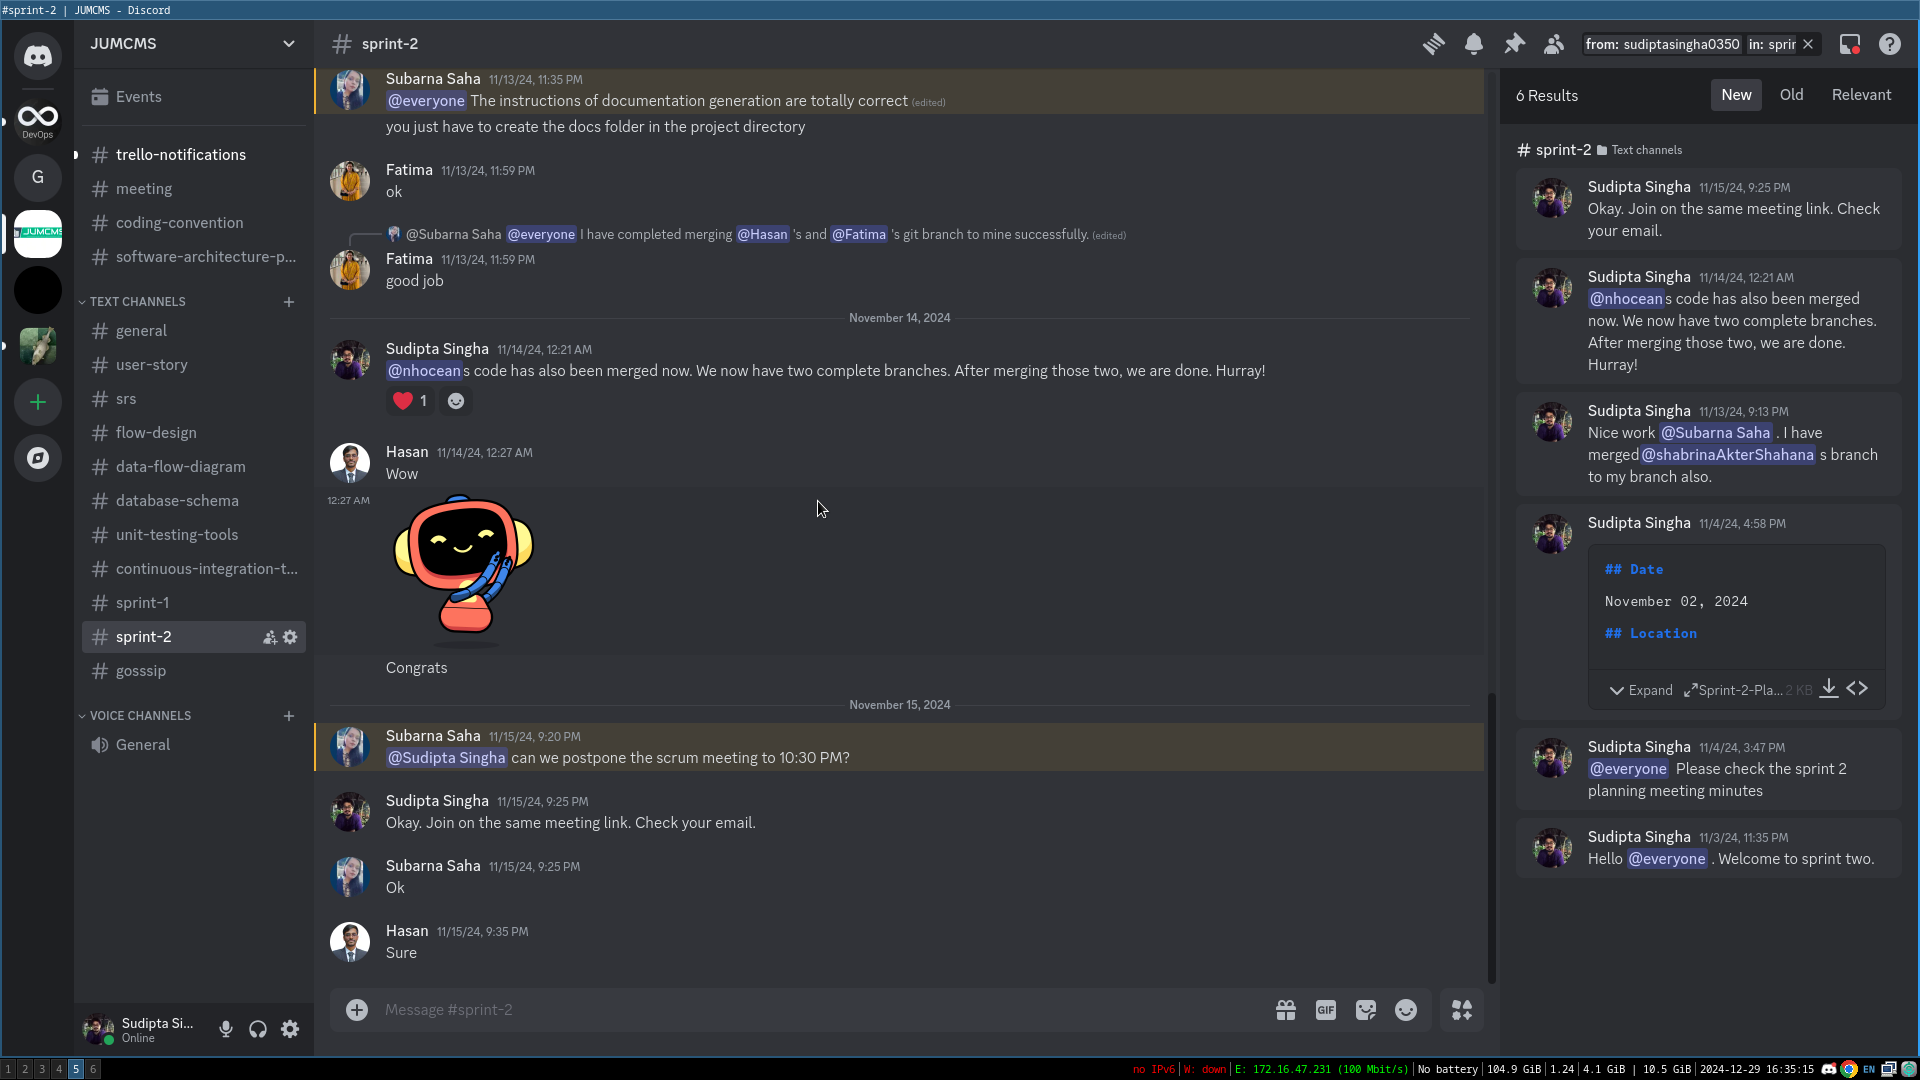
\includegraphics[width=0.8\textwidth]{images/discord_sprint2.png}
    \caption{Discord conversation for sprint 2}
    \label{fig:discordsprint2}
\end{figure}


\begin{figure}[H]
    \centering
    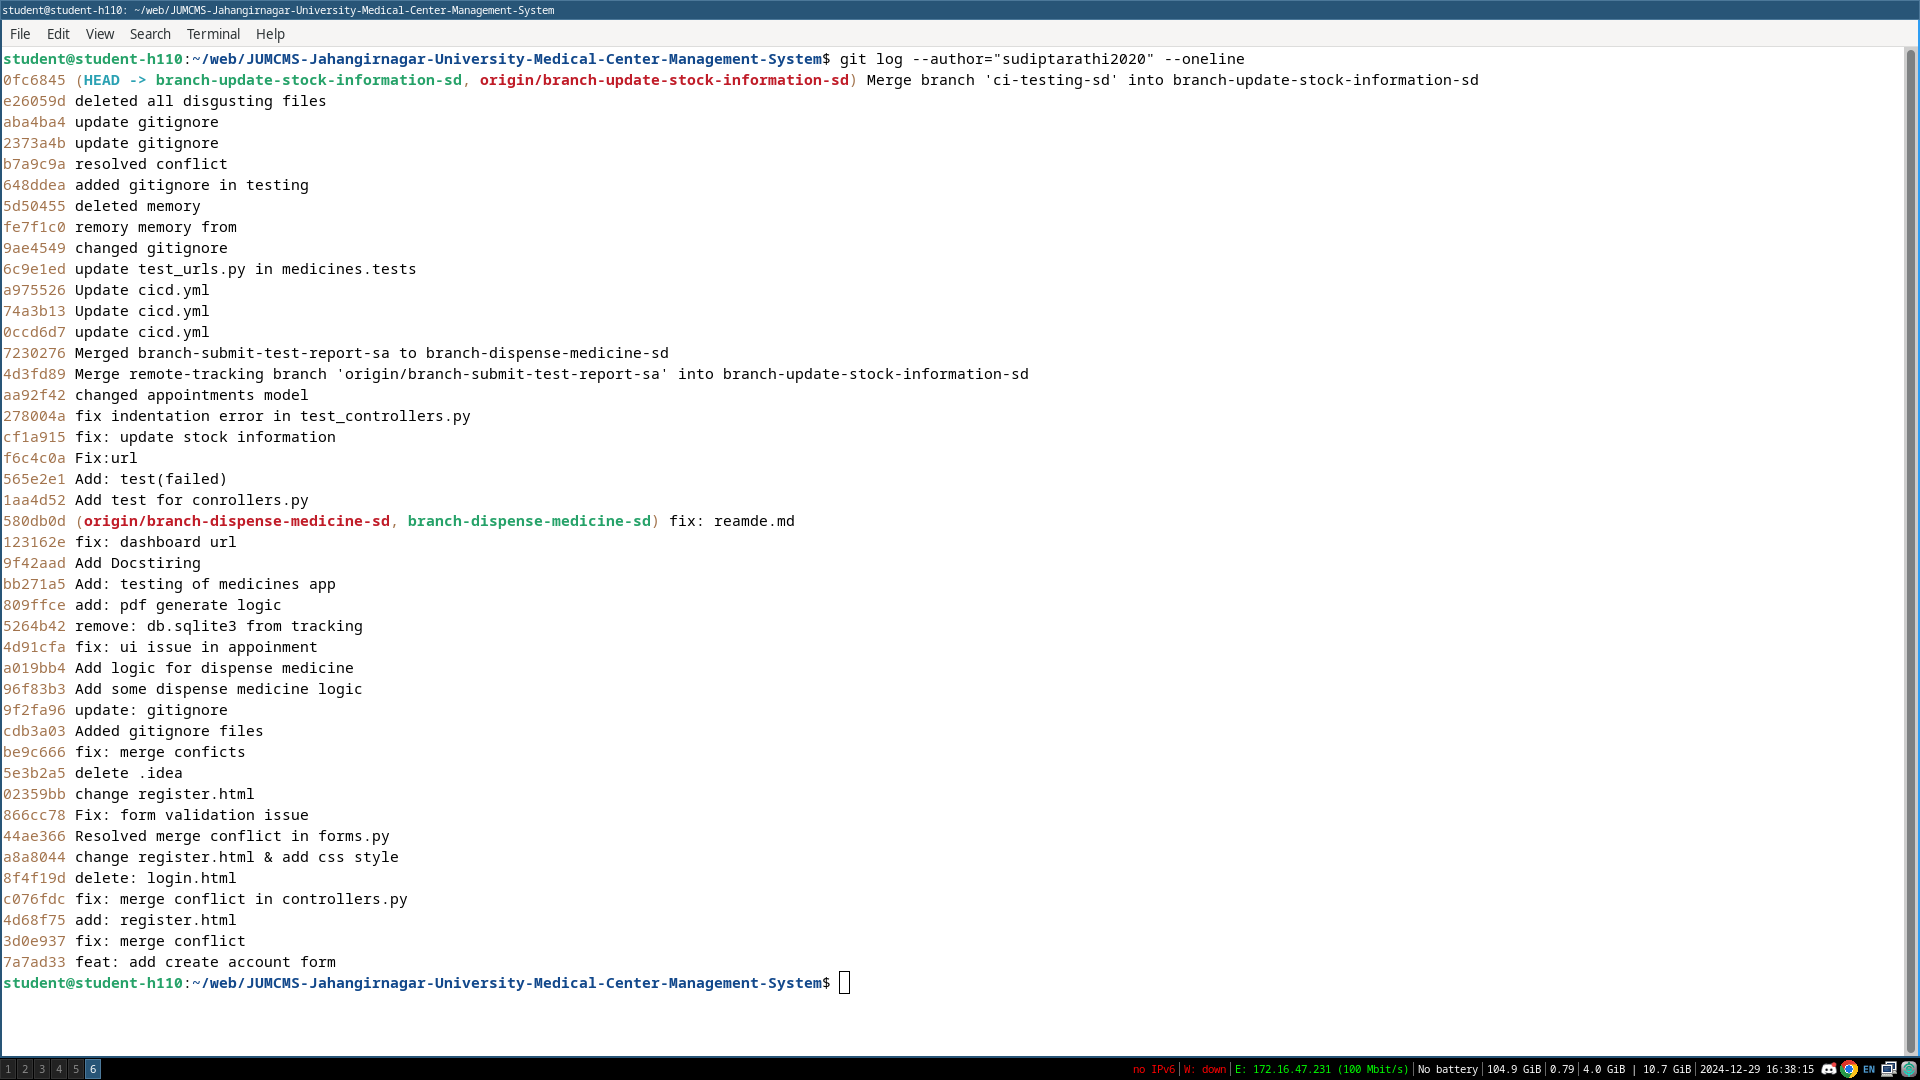
\includegraphics[width=0.8\textwidth]{images/git_sprint2.png}
    \caption{Git log for sprint 2}
    \label{fig:gitsprint2}
\end{figure}


\begin{figure}[H]
    \centering
    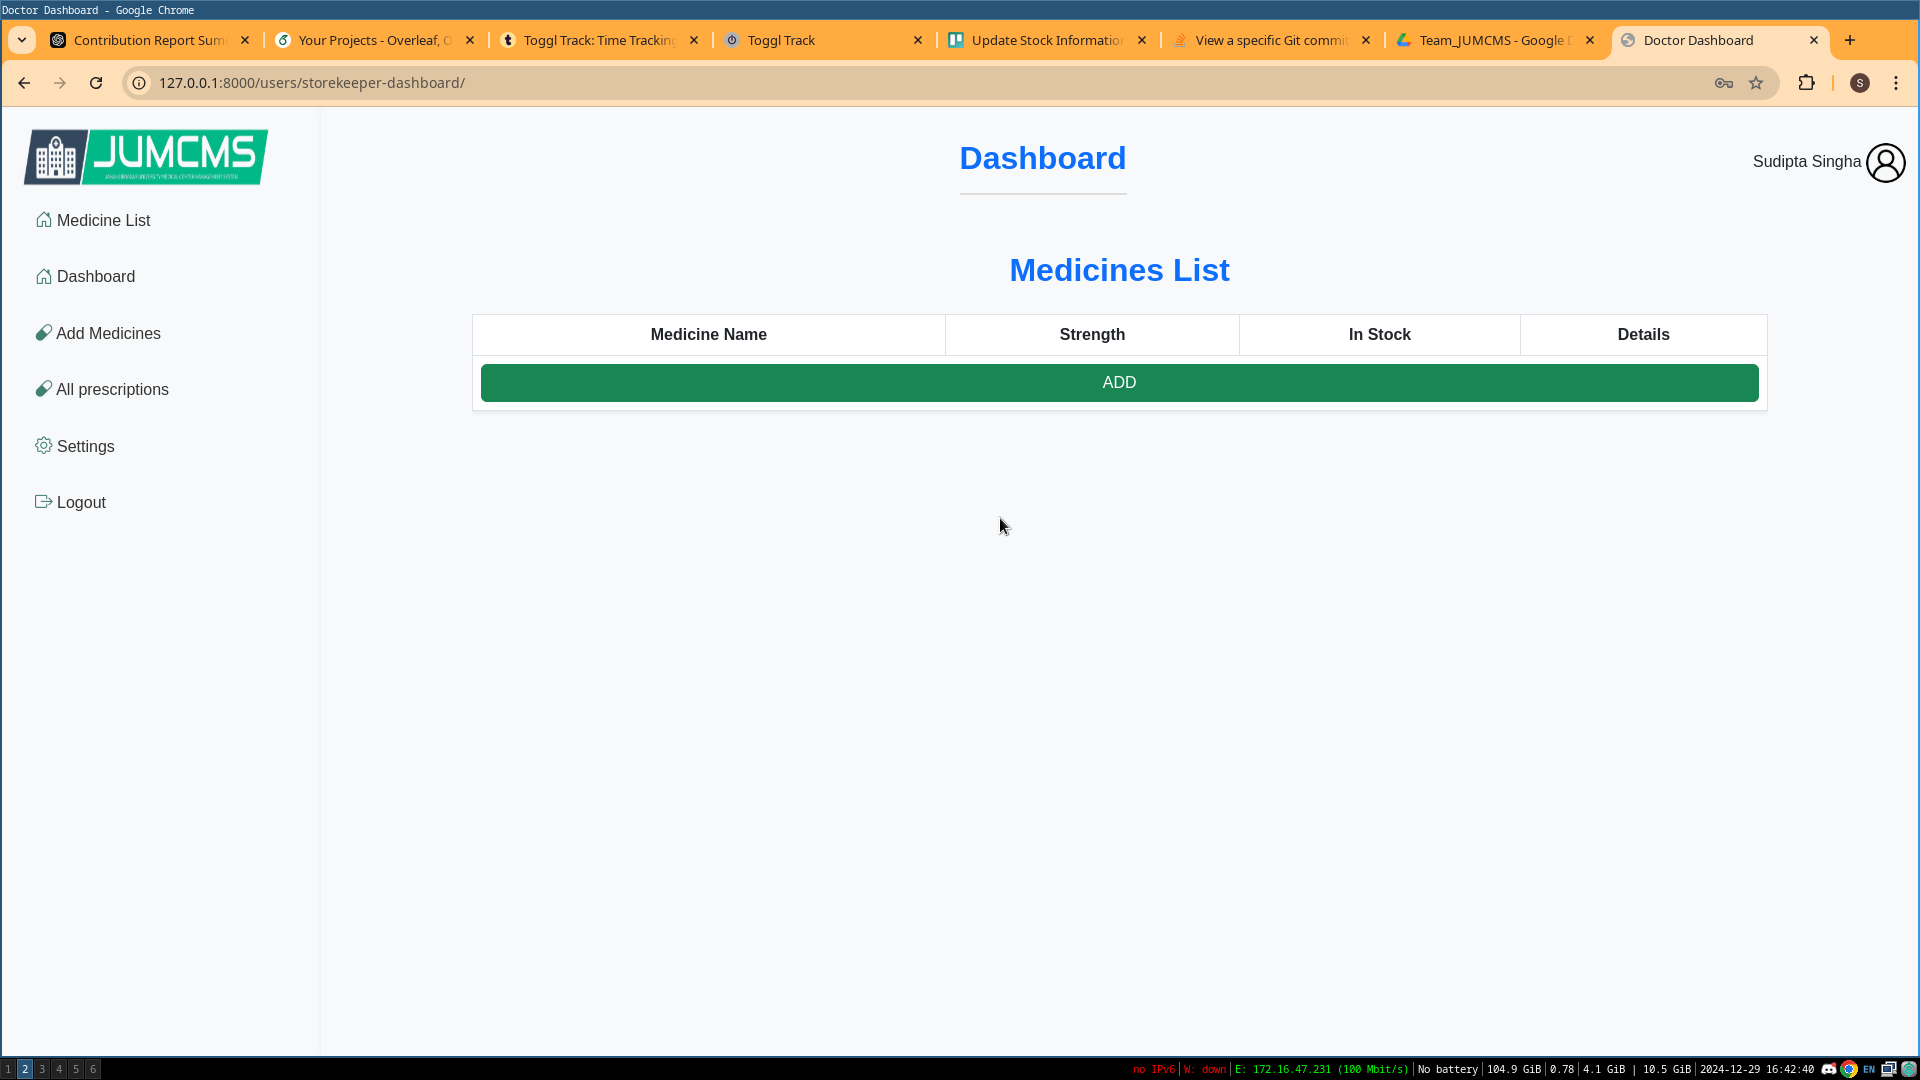
\includegraphics[width=0.8\textwidth]{images/spr2output1.png}
    \caption{Output for Update stock information}
    \label{fig:sp2out1}
\end{figure}


\begin{figure}[H]
    \centering
    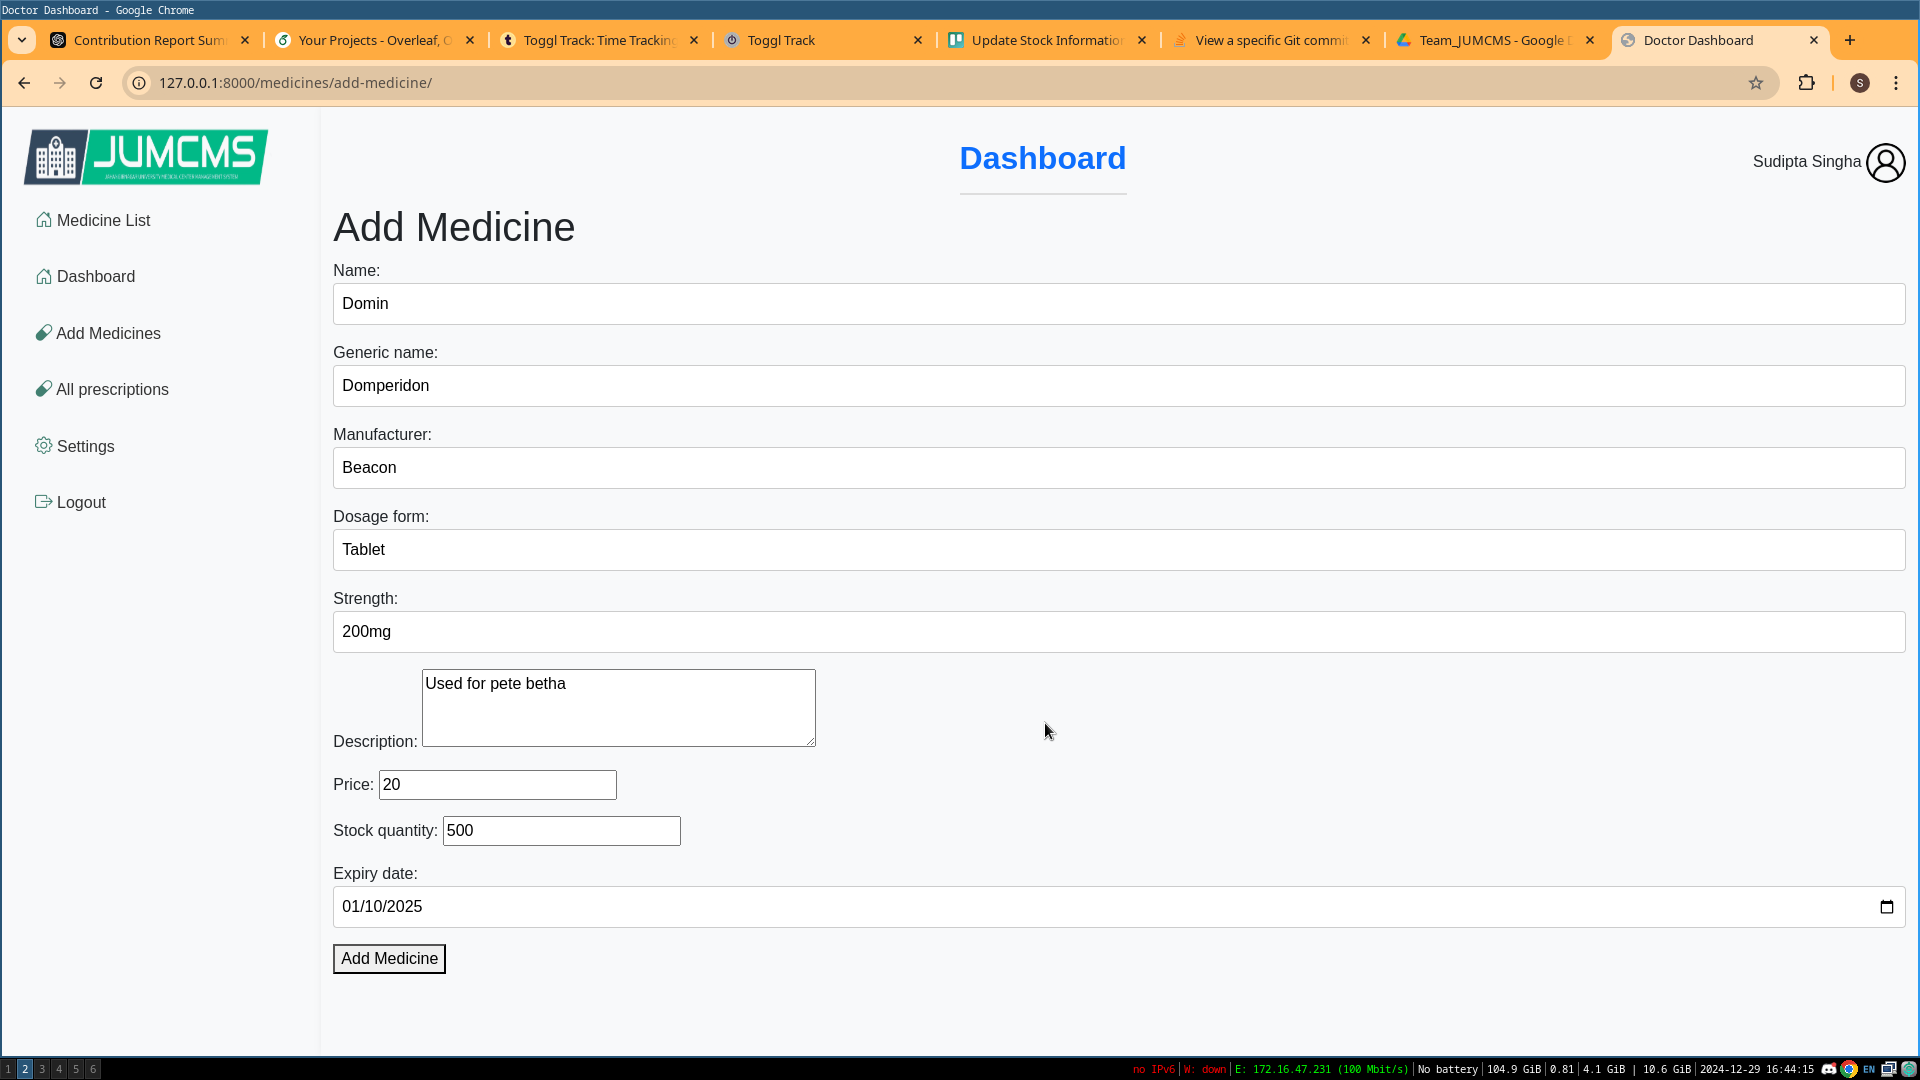
\includegraphics[width=0.8\textwidth]{images/spr2output2.png}
    \caption{output for update stock information}
    \label{fig:sp2out2}
\end{figure}


\begin{figure}[H]
    \centering
    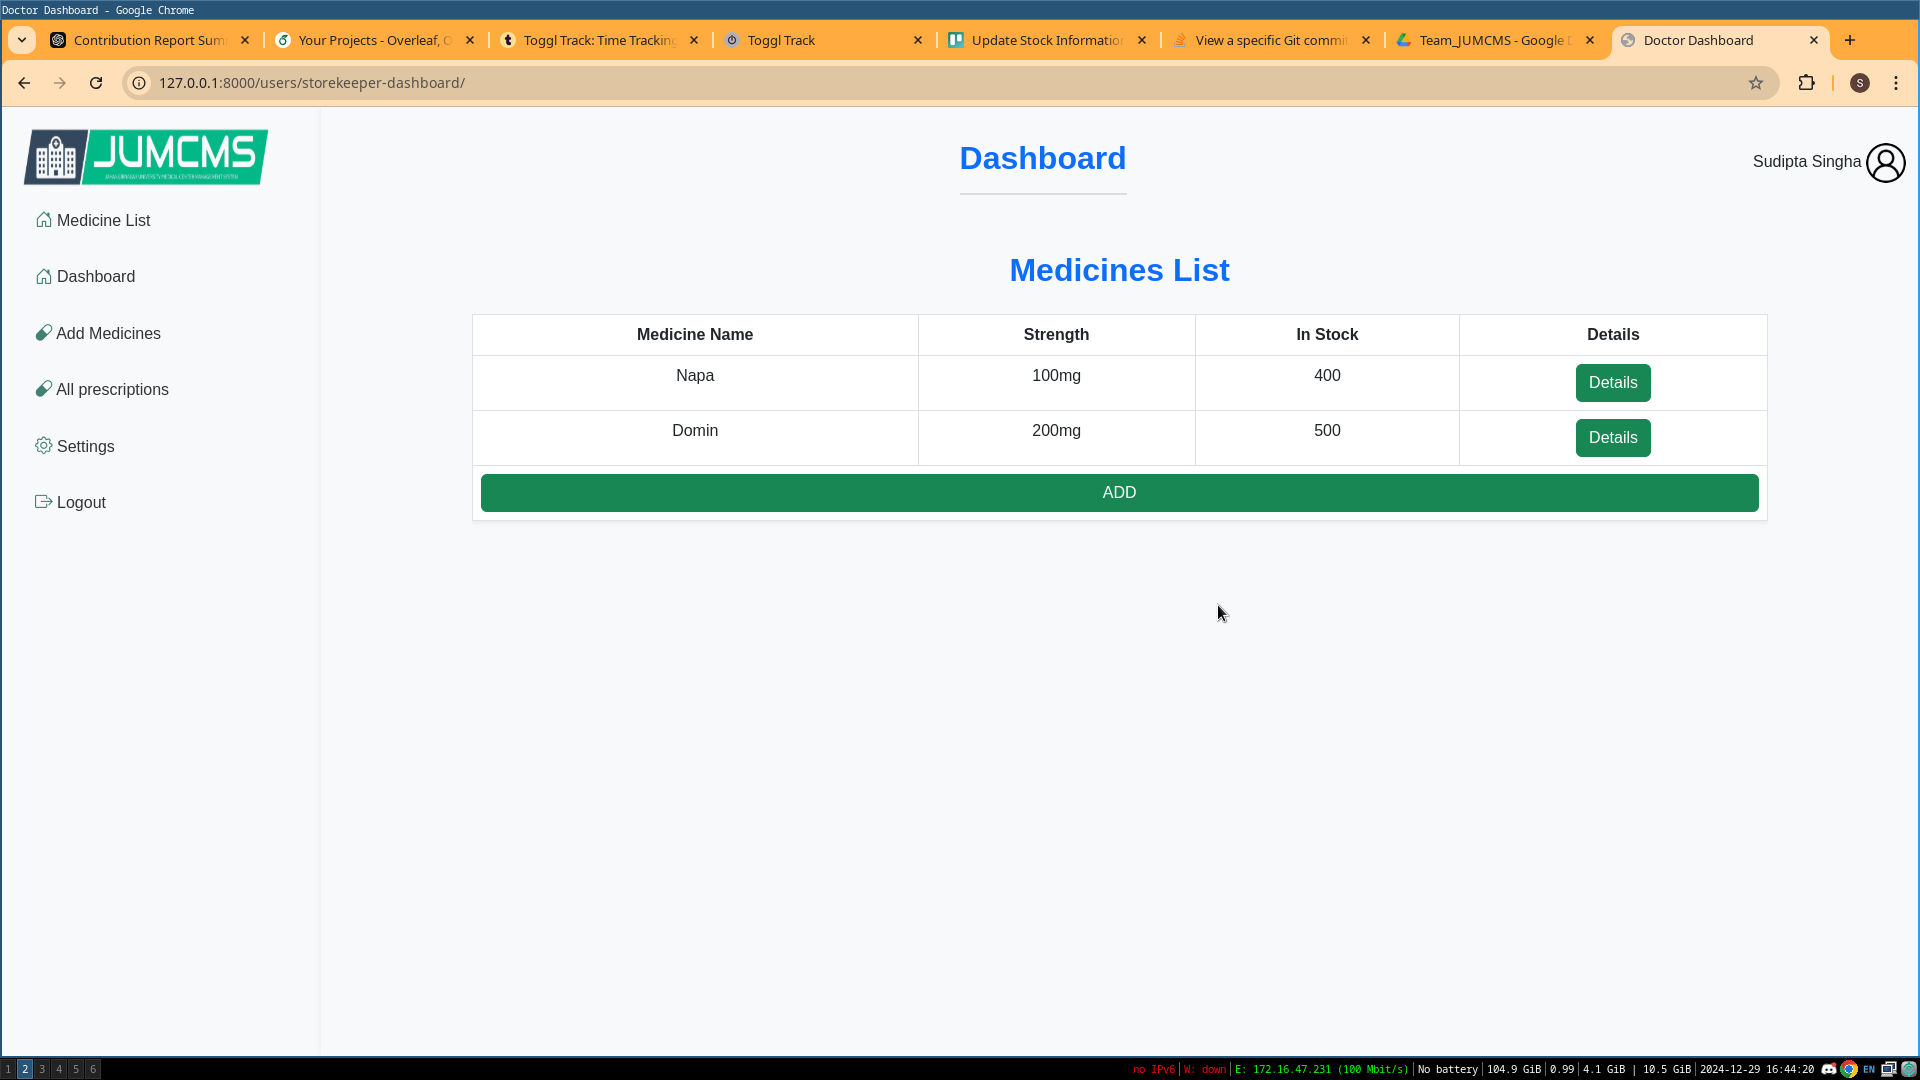
\includegraphics[width=0.8\textwidth]{images/spr2output3.png}
    \caption{Output for update stock information}
    \label{fig:sp2out3}
\end{figure}


\subsection{Integration}
\begin{itemize}
    \item Merged my branch with shabrina shahanas branch and Nahians branch
    \item Merged to main branch
    \item Create pull request
    \item Run github actions ci tool
\end{itemize}

\begin{figure}[H]
    \centering
    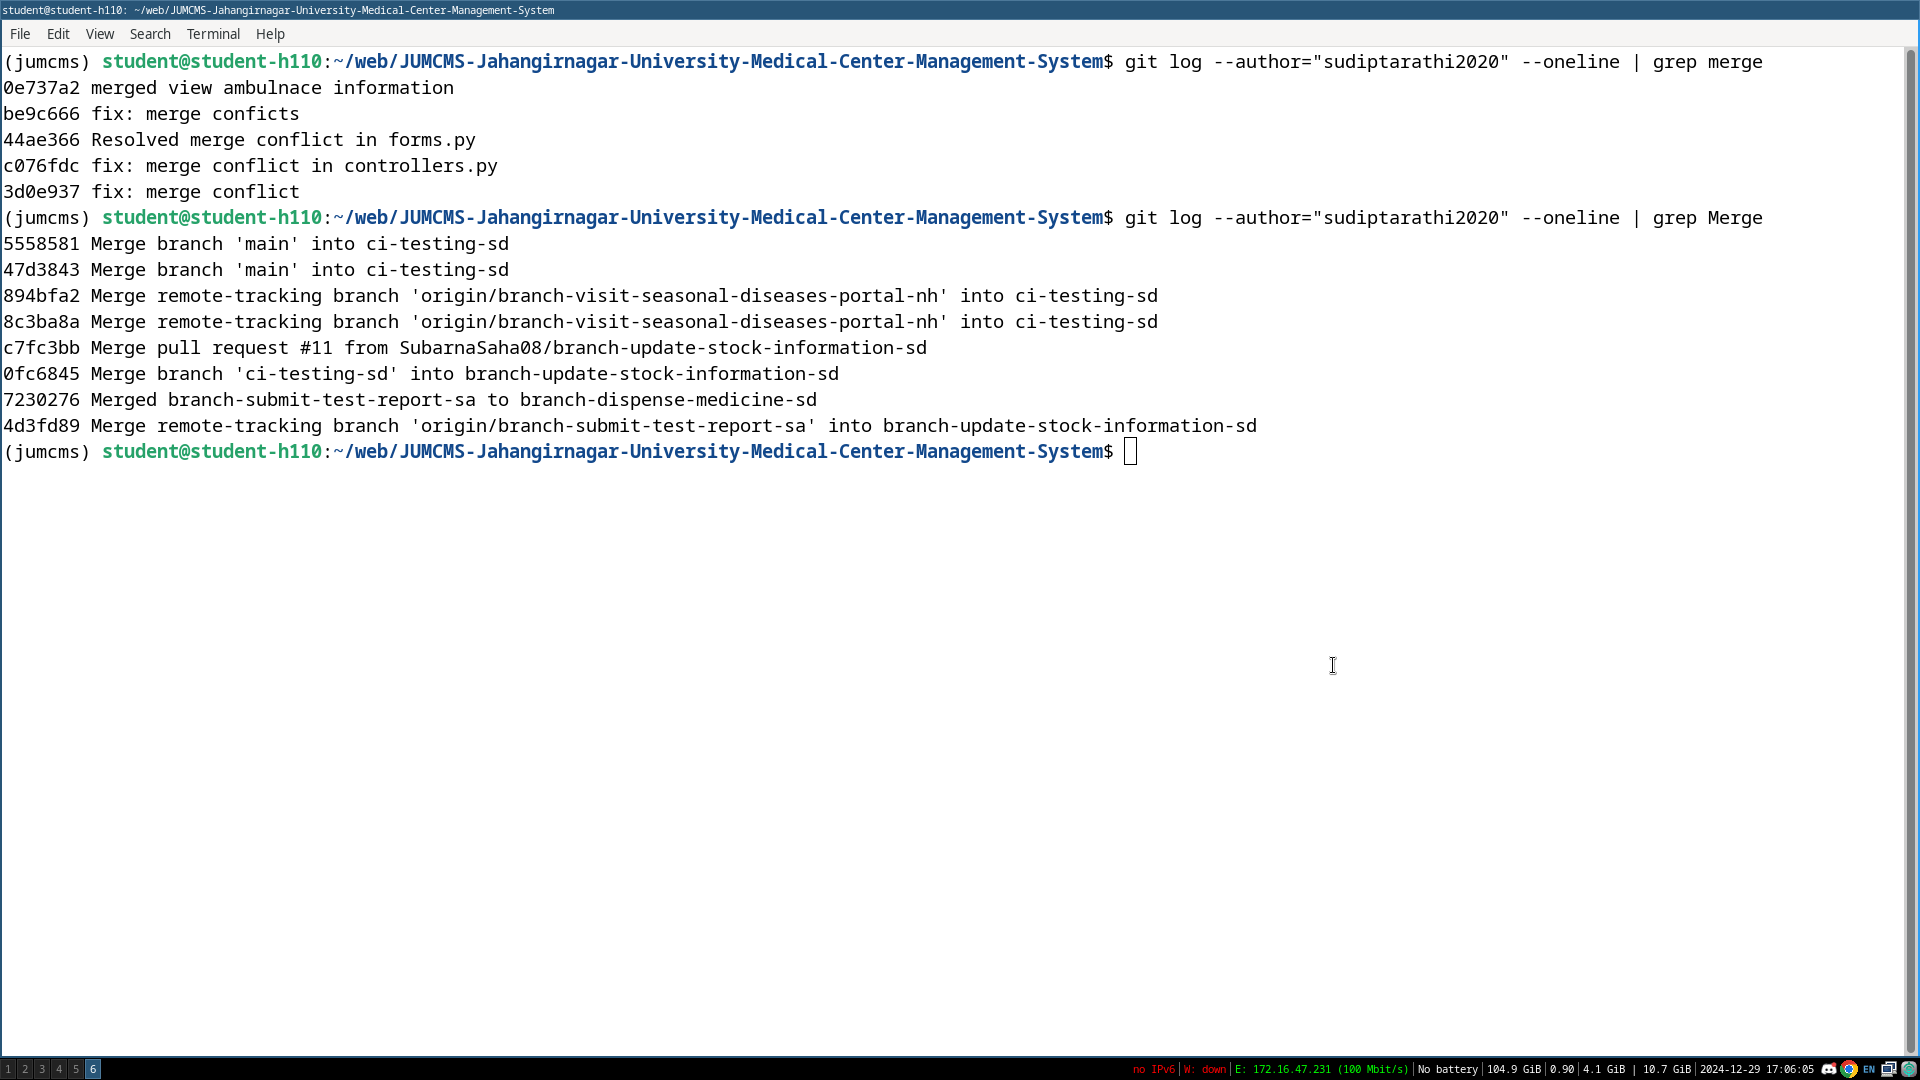
\includegraphics[width=0.8\textwidth]{images/merge.png}
    \caption{Solving merge conflics and merge to main branch}
    \label{fig:merge}
\end{figure}


\begin{figure}[H]
    \centering
    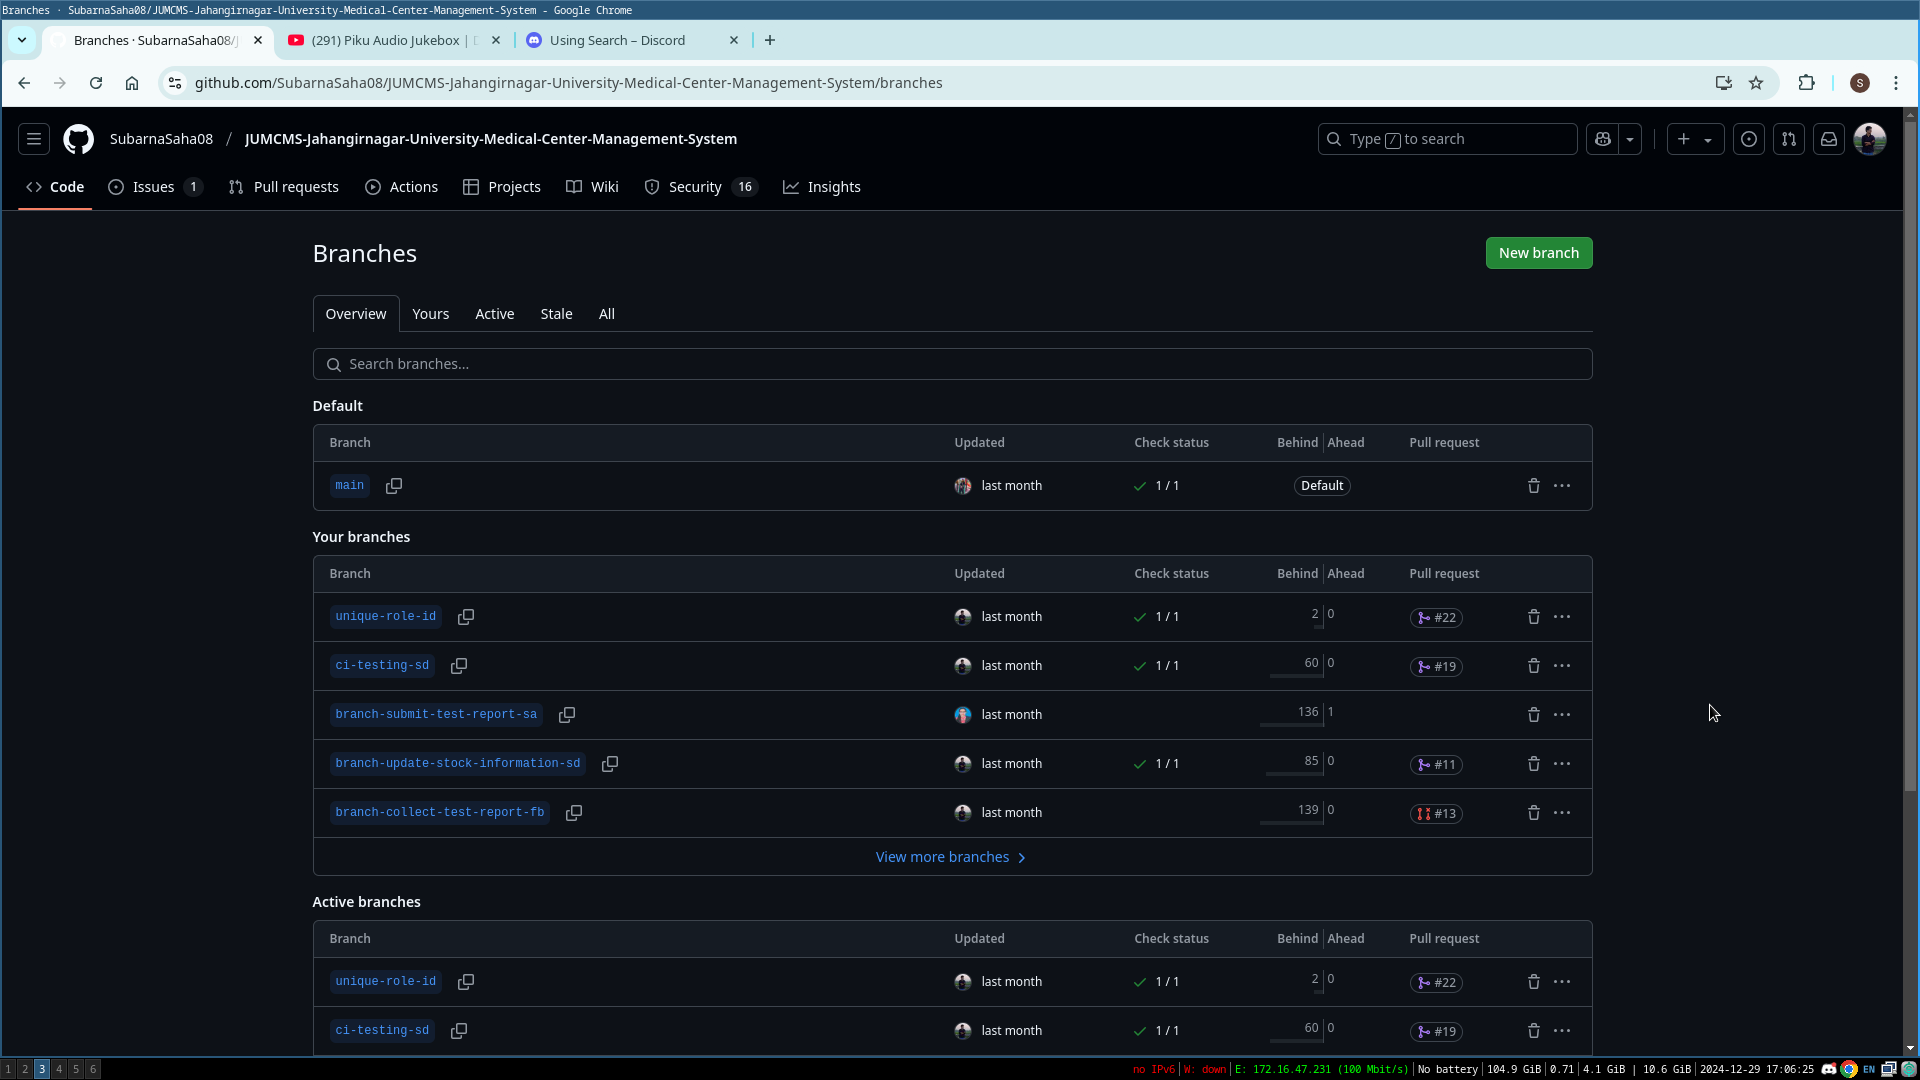
\includegraphics[width=0.8\textwidth]{images/mybranch.png}
    \caption{My branches}
    \label{fig:branches}
\end{figure}


\begin{figure}[H]
    \centering
    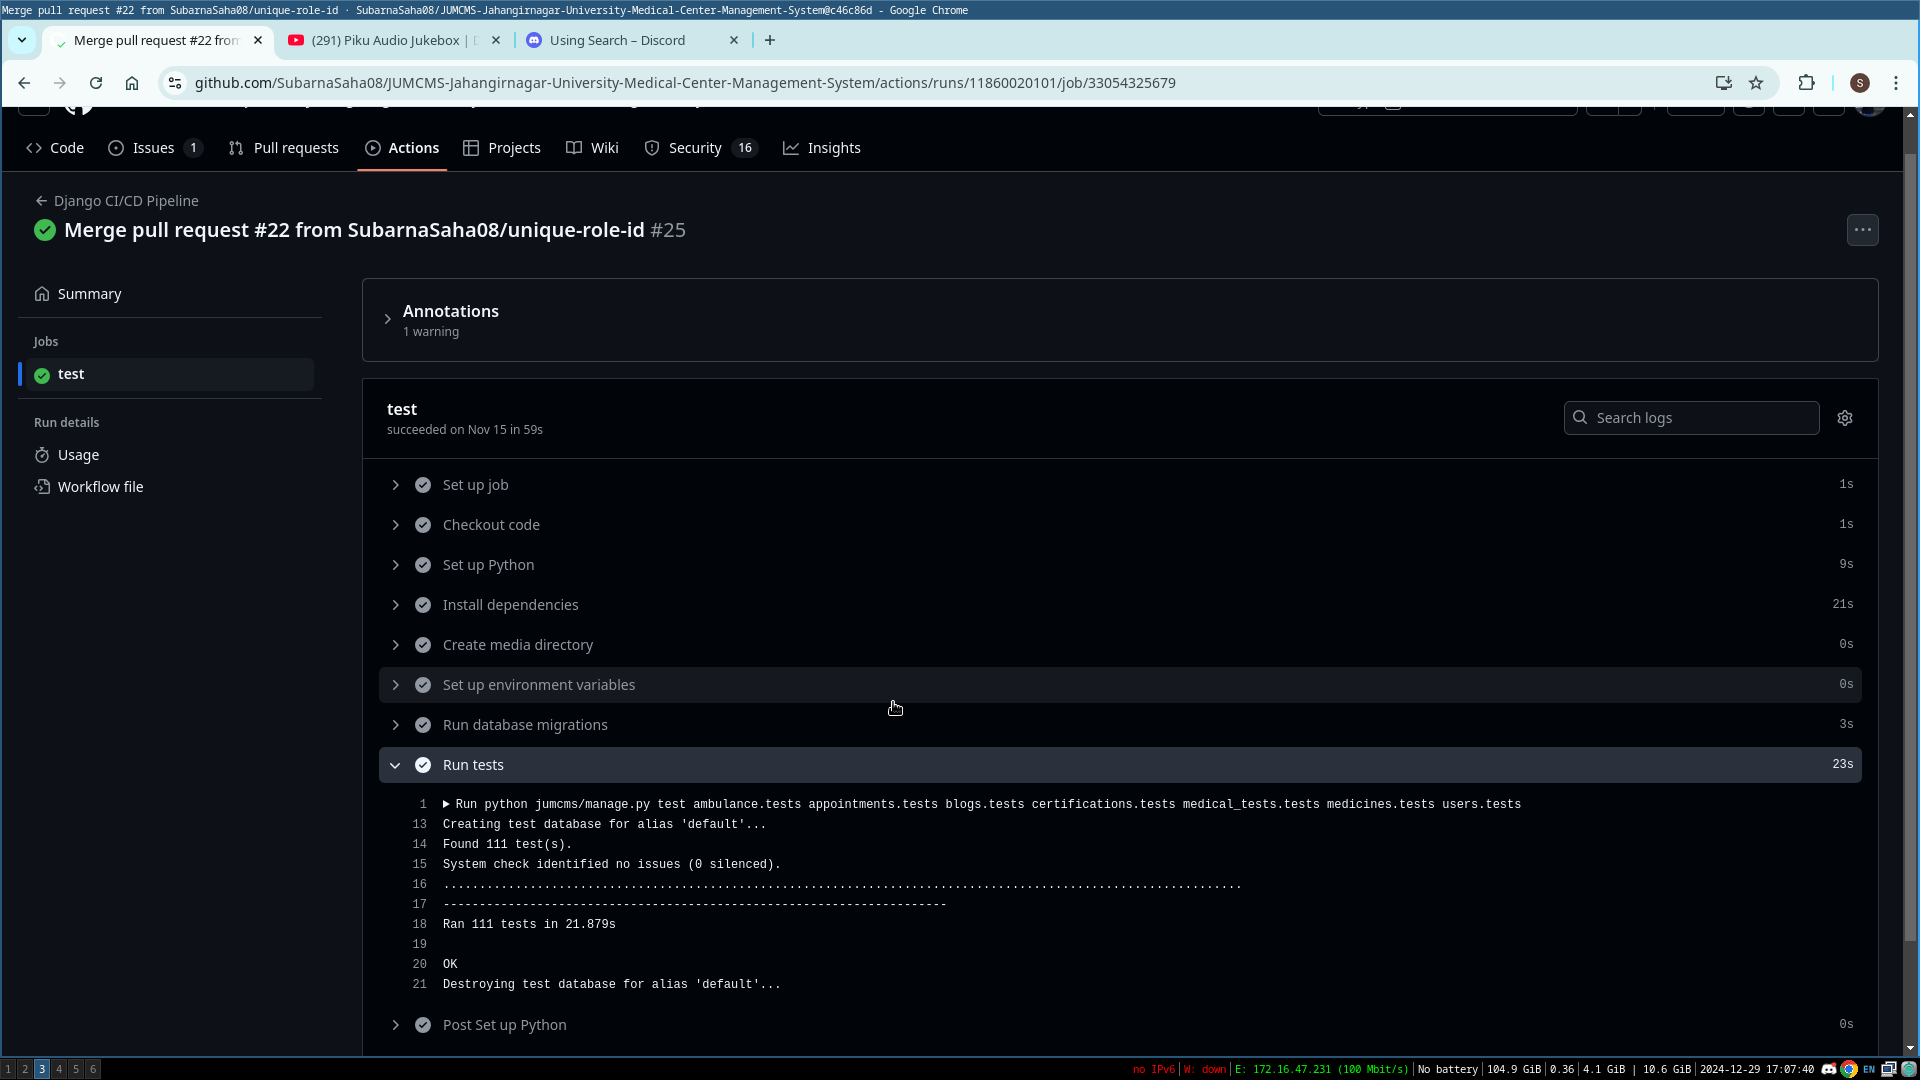
\includegraphics[width=0.8\textwidth]{images/githubaction.png}
    \caption{Github actions}
    \label{fig:cicd.yml}
\end{figure}


\subsection{Role}
In Sprint 2, I took on the role of Scrum Master, which involved additional responsibilities to ensure the
team’s success. These responsibilities included:
\begin{enumerate}
    \item Facilitating Scrum Meetings:
        \begin{itemize}
            \item Organized and moderated daily stand-ups, sprint planning, sprint review, and retrospective meetings.
            \item Ensured meetings stayed focused and productive, addressing blockers and maintaining progress.
        \end{itemize}
    \item Monitoring Progress:
        \begin{itemize}
            \item Tracked the team’s progress using project management tools (e.g., Toggl) and ensured tasks were completed on schedule.
            \item Maintained the sprint backlog, ensuring transparency and clarity in task assignments
        \end{itemize}
    \item Supporting Team Members:
        \begin{itemize}
            \item Assisted team members with technical challenges and provided guidance to ensure the quality of deliverables.
        \end{itemize}
\end{enumerate}
\newpage
\section{Reflection}
Through this project, I gained valuable experience in full-stack development, particularly with Django’s
framework. Collaborating with my team taught me the importance of effective communication and the use of agile
methodologies for project management. Tools such as Git and Jira were instrumental in tracking progress and
ensuring seamless collaboration.

The project’s success relied heavily on the integration of diverse tools and practices. For instance, Django’s
ORM simplified database interactions, and our adoption of a modular approach to development enhanced
maintainability. The team’s collaborative spirit and commitment were pivotal in achieving our goals.

Furthermore, I explored effective ways to contribute to the project’s codebase by engaging in discussions,
attending scrums, and researching best practices. The inclusion of screenshots of Git logs, my GitHub
contribution graph, functional code snippets, and website interfaces will provide additional context and
evidence of my involvement.

Overall, this project has been a significant learning opportunity, equipping me with skills that will be
valuable in future endeavors.
\end{document}

